\documentclass{article}
\usepackage{pgfplots}
\pgfplotsset{compat=1.18}
\usepackage{multicol}
\usepackage{tikzit}
\input{PhysiksStyle.tikzstyles}
\usepackage{geometry}
\usepackage{titlesec}
\titlespacing*{\subsubsection}{0pt}{1.2ex}{.1ex plus .2ex minus .2ex}
\usepackage{amsmath}
\usepackage{amsfonts}
\usepackage{amssymb}
\geometry{margin=1.5cm}
\author{Benjamin Dropmann}
\hbadness=10001
\vfuzz=10001pt
\newcommand{\mspc}{\hspace{0.4cm}}
\newcommand{\experiment}{\\[2ex]\textbf{Experiment }}

\begin{document}
\begin{abstract}
\subsection{Bonusprogramm}
12 serien* 5 punkte / serie$\rightarrow$ 60 punkte\begin{itemize}
\item[\textbullet]{0-19 Kein bonus}
\item[\textbullet]{20-39 Lineare interpolation}
\item[\textbullet]{$>$40 maximaler bonus 39, 40 schon maximler bonu}
\end{itemize}
\end{abstract}
\section{Wellen}
\subsection{Federwelle} Gutes model für eine Festkoper, Transversale Anregung, senkrecht zur länge, Longitundonale Anregung, entlang der  längle des feder dings. (Elektromagnetik schwer da es in beide richtungen geht). Es gelten Folgende Bedingungen für die federwelle:
\begin{itemize}
\item[\textbullet]Jede masse Schwingt um ihre ruhelage, (wie eine Pendel)
\item[\textbullet]Jede masse bleibt in ruhe bis die welle sie erreicht
\item[\textbullet]Ruckrehr zur ruhelage
\end{itemize}
\subsubsection{Amplitude} der Welle $\xi(x,t)$ ($x$ : Ort fur die Seilwelle, $t$ zeit)
\subsubsection{Dispersion}: Form des wellenpakets der anregung bleibt unverändert
$\xi(x,t=0)=f(x)$ $f(x)$ ist die form des wellenpakets\\$x-a$ fuhrt zu einer translation der Wele ohne ändergun seiner form:
\[c\rightarrow x-a\rightarrow \xi(x-a,t=0)\rightarrow (x+a)\]
\[a=vt \rightarrow f(x\pm vt)\]
\[\xi(x,t)=f(x\pm vt\] $v$ ist hier die \textbf{Phasengeschwindigkeit} der Welle.
\subsubsection{Harmonische Wellen} Vom Harmonischen Oszillator, Wellengleichung herleiten, allgeimene wellengleichung finden. Eine Harmonische Welle ist eine sinus (cosinus ist besser) kurve
\[\xi(x,t)=\xi_0\cdot\sin(k(x\pm vt=f(x\pm vt)\]
\[\text{Wellenzahl }k(x+\lambda)=kx+2\pi \rightarrow k\lambda = 2\pi \rightarrow k=\frac{2\pi}{\lambda}\]
$k$ ist die Wellenzahl (so dass was im sinus ist dimensionslos ist)  \[\lambda:{Wellenlange}\]
In zwei dimensionen ist $k$ä ist ein vektor und zeigt uns die wellen direktion aus (longitude, oder senkrecht)
\\Kreisfrequenz: $\omega=2\pi\nu=2\pi\frac{1}{T}$ Wo $T$ die Periode ist.\\$\xi(x,t)=\xi_0\sim(k(x\pm vt))=\sin(kx+kvt)=\xi_0\sin(kx\pm\omega t)$

\subsubsection{Wellenglaichung in einer Dimension}
\[\xi(x,t)=\xi_0e^{i(kx\pm \omega t}\]
wir leiten nach der zeit ab:
\[\frac{\delta\xi}{\delta t}=\xi_0(-kv)cos(k(x-vt))\]
\[\frac{\delta^2\xi}{\delta^2t}=\xi_0(-kv)^2sin(k(x-vt))\]
ncahc dem ort ableiten
\[\frac{\delta\xi}{\delta x}=\xi_0kcos(k(x-vt))\]
\[\frac{\delta^2\xi}{\delta^2x}=\xi_0k^2sin(k(x-vt))\]
Zusammestellen $\frac{\\delta^2\xi}{\delta^2t}=v^2\frac{\\delta^2\xi}{\delta^2x}$
\[\frac{\delta^2\xi}{\delta^2t}-v^2\frac{\\delta^2\xi}{\delta^2x}=0\]
Wie sieht dann die algemeine lösung aus?
\[\xi(x,t)=f(x-vt)+g(x+vt)\]
Ableitung nach der Zeit
\[\frac{\delta\xi}{\delta t}=\frac{\delta f(x-vt)}{\delta t}+\frac{\delta f(x+vt}{\delta t}=\frac{\delta f(\alpha(x,t)}{\delta t}+\frac{\delta g(\beta(x,t)}{\delta t}\]
Weiter und weiter ableiten und herumschreiben:
\[\frac{\delta f}{\delta \alpha}(\alpha(-v)+\frac{g(\beta)}{\delta \beta}(\beta(v)\]
Für die zweite ableitung gilt diese hergehensweise auch, und wir finden dass die gleicung oben erfüllt ist und dass folgende gleichung gilt:
\[\frac{\delta^2\xi}{\delta^2t}-v^2\frac{\delta^2\xi}{\delta^2x}=0\]
Gute frage: jede sinusfunktion erfullt das; wir haben nur angenommen dass $x$ und $t$ einen anhang ($f$ in diesen fall) haben
\experiment DNA dings, sehr wenig reibug zwischung elemente $\rightarrow$ rucktreibendende kraft sehr gering. Auch reflektion. 

\subsubsection{Transversale Wellen}
\[\xi(z,t)=Af(z-vt)\]
Diesmal ist $k$  aber ein Vektor
\[xi(z,t)=A\cos(kz\omega t)\hat{x}\]
Anhange zur spannung(seilwelle) Seilwelle$\rightarrow$ Wellengleichung
Wir nehmen viele kliene massenelemente den seil entlang, Dann haben wir zwei kräfte, den seil hoch/entlang und die spannung des seils/nach unten. Wir haben jetzt für eine massen element zwei funktionen $xi(x)$ und $\xi(x+dx)$ Wir brauchen also der unterschid zwischen diese zwei kräfte, die nicht entgegengesetzt sind wegen der breite des massenelements.
\[\Delta S_y=S\sin(\alpha')-S\sin(\alpha)\]
Herumdingen
\[\Delta S_y=S\frac{\delta^2\xi}{\delta x^2} dx\]
Ich habe verpasst Elastizität modul?
\subsubsection{Räumliche verteilung von Wellen}
\[\xi(x,y,z,t)=Af(kz-\omega t)\]
Transversale Welle: Polarisationsrichtung (in x oder y schwingen, transversal aber anders)
\[A=\begin{pmatrix}A_x\\A_y\end{pmatrix}\mspc \xi(t)=\begin{pmatrix}A_x\\A_y\end{pmatrix}\cdot e^{ikz-\omega t}\]
Die wellenzahl wird jetzt zu einem Vektor der beschreibt in welcher richtung diese welle sich ausbretet. 
\[\xi(r, t)=Ae^{i(kr-\omega t)}\] wobei $k=\begin{pmatrix}0\\0\\k_z\end{pmatrix}$
\subsection{Wellengleichung in drei dimensionen}
\[\frac{1}{v^2}\frac{\delta^2\xi}{\delta t^2}-\frac{\delta^2\xi}{\delta x^2}-\frac{\delta^2\xi}{\delta y^2}-\frac{\delta^2\xi}{\delta z^2}=0\]
Laplace operator $\Delta=\nabla^2=\left(\frac{\delta}{\delta x},\frac{\delta}{\delta x},\frac{\delta}{\delta x}\right)\begin{pmatrix}\delta/\delta x\\\delta/\delta y\\\delta/\delta z\end{pmatrix}$ Also es gilt \[\frac{1}{v^2}\frac{\delta^2\vec{\xi}}{\delta t^2}(x,y,z,t)-\Delta\vec{\xi}=0\]
\subsection{Kugelwellen}
Beispiel punktformige Lichtquelle. Hier ist $k$ nicht mehr wohldefiniert, da die welle sich in alle richtungen ausbreitet.
\[\vec{\xi}_0\cdot e^{i(\vec{k}\vec{r}-\omega t}\]
\[\frac{\delta \vec{\xi}}{\delta x}=ikxe^{i(\vec{k}\vec{r}- \omega t}\]
In alle richtungen und zweimal ableiten, und wir finden:
\[\Delta\vec{\xi}(\vec{r},t)=-k^2\vec{\xi}(\vec{r},t)\]
Und dann dasselbe mit der zeit:
\[\frac{1}{v^2}\frac{\delta^2\vec{\xi}}{\delta t^2}-\Delta\vec{\xi}=\xi\left[-\frac{\omega^2}{v^2}+k^2\right]\vec{\xi}\mspc v=\frac{\omega}{k}\]
Mit der Kugel symmetrie $\Delta = \frac{\delta^2}{\delta x^2}+\frac{\delta^2}{\delta y^2}+\frac{\delta^2}{\delta z^2}$
bekommen wir dann 
\[\frac{\delta \phi}{\delta x}=\left(\frac{\delta r}{\delta x}\frac{\delta}{\delta r}+\frac{\delta \theta}{\delta x}\frac{\delta}{\delta \theta}+\frac{\delta \phi}{\delta x}\frac{\delta}{\delta \phi}\right)\phi\]
\[\frac{\delta r}{\delta x}=\sin(\theta)\cos(\phi)\]
\[\frac{\delta\theta}{\delta x}=\frac{\delta}{\delta x}\left[\arccos\left(\frac{z}{r}\right)\right]=\frac{1}{\sqrt{1-\frac{z^2}{r^2}}}\frac{\delta}{\delta x}\frac{z}{r}=\frac{1}{\sqrt{1-\frac{z^2}{r^2}}}\left(-\frac{1}{2}\frac{1}{r^3}2xz\right)\]
\[=\frac{1}{r}\cos(\theta)\cos(\phi)\]
Dasselbe geht jetzt mit $\frac{\delta \phi}{\delta x}$ (Schreibe ich nicht hin)
\subsection{Kugelwellen, Wellengleichungen in 3d}$\vec{k}\cdot\vec{r}= |\vec{k}|\cdot|\vec{r}|=k\cdot r$ Da $k$ und $r$ immer parallel laufen (dank der Kugelsymmetrie)
\[\vec{\xi}(r,t)=\frac{\vec{A}_1}{r}f_1(kr-\omega t)+\frac{\vec{A}_2}{r}f_2(kr-\omega t)\]
Diese lösung erfullt die differentialgleichung.
\subsection{Energietransport} Die Geschwindigketi eines massenstücks $v=\frac{\delta \xi(\vec{r},t}{\delta t}$\\
Die kinetische energie dieses massenstuck $dT=\frac{1}{2}\left(\frac{\delta \xi}{\delta t}\right)^2 dm$
Energie dichte $\frac{dT}{dV}$
\\
Elastische energie:
\[E_{el}=\int_0^{\Delta l}(\Delta l')d(\Delta l')=A\int_0^{\Delta l}E\frac{\Delta l^2}{l}=\frac{1}{2}(A\cdot l)E\left(\frac{\Delta l}{l}\right)^2\]
\[\frac{\Delta l}{l}=\frac{\delta \xi}{\delta x}\Rightarrow\frac{1}{2}E\left(\frac{\delta \xi}{\delta x}\right)^2\]
Energie dichte:
\[\frac{dT}{dV}=\frac{1}{2}\rho v^2 f'^2\]
\[\frac{dE_{el}}{dV}=\frac{1}{2}Ef'^2\]
Pro volumen gerechnet ist die elastische und kinetische energie dieselbe. Die Gesamtenergie ist alow $\frac{dW}{dV}=\rho v^2f'^2$\\
\subsection{Wellenfunction $\xi$}
\[\xi(x,t)=\]
Die Form einer welle: $f(x)=\xi(x,t=0)$ ist der initiale gefrorene status einer Welle. Für jetzt, ist die Form konstant (dämpfungen sind benachlässigt). Wegen der Form der Welle, ist ort und Zeit nicht unabhängig, da die Form der Welle nur den Ort definiert bei einer konstanter Zeit.\\
Nach eine Zeit hat sich die Welle bus zum punkt $x\pm vt$ ausbreitet, wobeir $v$ die Wellengeschwindigkeit ist. Die Wellenfunktion ist also\[\xi(x,t)=f(x\pm vt)\]
\subsection{Harmonische Welle}
Eine harmonische Welle ist beschrieben durch ein sinus oder ein cosinus:\[\xi(x,t)=A\cdot\sin(k(x\pm vt)\] wobei $k$ die Wellenzahl (später Wellenvektor) $\left[\frac{1}{m}\right]$, ist, $A$ die Amplitude. Es gilt $k=\frac{2\pi}{\lambda}$ wo lambda die Wellenlänge ist. Also man kann die folgende vereinfachung machen:
\[k(x\pm vt)=kx+kvt=kx+\omega t\]
wobei $\omega$ die Kreisfrequenz ist.\\
\subsection{Wellengleichung}
Wir leiten nahc der Zeit ab
\[\frac{\delta\xi}{\delta t}=A(-\omega)\cos(kx-\omega t)\]
\[\frac{\delta^2 \xi}{\delta t^2}=a-\omega^2A\sin(kx-\omega t)\]
Und jetzt nach dem Ort:
\[\frac{\delta\xi}{\delta x}=Ak\cos(kx-\omega t)\]
\[\frac{\delta^2 \xi}{\delta x^2}=-k^2A\sin(kx-\omega t)\]
Wie setzen dies zusammen und Bekommen:
\[=\frac{\omega^2}{k^2}\frac{\delta^2\xi}{\delta x}=v^2\frac{\delta^2\xi}{\delta x^2}\]
\[\frac{\delta^2 \xi}{\delta t^2}-v^2\frac{\delta^2\xi}{\delta x^2}\]
Die Allgemeine Lösung olgt folgender Form:
\[f(x-vt)-g(x+vt)\]
\subsubsection{Arten von Wellenverbreitung}
\begin{itemize}
\item{Transversalwelle: Auslenkung senkrecht zur geschwindigkeit}
\item{Longitudonalwell, die Auslenkung ist parallel zur ausbreitung der Welle}
\end{itemize}
\subsubsection{Energietransport einer Welle}
Eine welle transportiert kinetische und elastische energie, die Beträge dieser beiden einergien ist im volumen (flachenelement oder distanz) immer gleich.
\subsubsection{Tipps zur Serie 1}
\begin{itemize}
  \item[$1.1_a$]{Vollständige Wellenfunktion finden, (wichtige dingen oben sind hilfreich)}
\item[$1.1_b$]{Die orte einfch einsetzen und die trigonometrische vereinfachen mit den mathemathischen hilfsmitteln der formelsammlung}
\item[$1.2_a$]{Uhr und Lineal, so dass man zeiten und abständen messen kann. Welche gössen sind gegeben, und welche sin messbar? damit vereinfachen. Die Wellenlänge kann man (theoretisch messen) also mit der Wellenlänge die distanz ausrechen.}
\end{itemize}
\subsubsection{Stehende Welle} Die Stehende Welle ist einfach eine summe der Zwei wellen die sie aufführt.
\subsubsection{Reflection und Transmission} Transmission ist in derselben richtung als einkommende Welle, Reflektierte welle dagegen
\[\xi_A=Ae^{i(k_1x-\omega t)}\]
\[\xi_R=Ree^{i(-k_1x-\omega t +\delta_R)}\]
\[\xi_R=Te^{e(kx-\omega t +\delta_T)}\]
Wir konnen diese glaichungen mit zwei Parameter (zwei gleichungen) losen.
\newline Wir haben Zwei Bedingungen:
\newline Steigkeit\[lim_{x\rightarrow 0^-}(\xi_a+\xi_R)=lim_{x\rightarrow0^+}\xi_T\]
Und Kraftegleichgewicht:\[S_1\frac{\delta\xi_a}{\delta x}\left.\right|_{x=0}+\frac{\delta\xi_R}{\delta x}\left.\right|_{x=0}=\frac{\delta\xi_T}{\delta x}\left.\right|_{x=0}\]
\[A+Re^{i\delta_R}=Te^{i\delta_T}\]
Imaginärteil: $T\sin(\delta_T)=R\sin(\delta_R)$
\[Kraftgleichung\mspc AS_1k_1=TS_2k_2e^{i\delta_T}+RS_1k_1e^{i\delta_R}\]
\[TS_2k_2\sin(\delta_T)+RS_1k_1\sin(\delta_R)=0=T\sin(\delta_T(S_2k_2+S_1k_1))\]
Und wir bekommen
\[k_i=\frac{\omega}{v_i}\]
\[\alpha=\frac{S_2\delta_2}{S_1\delta_1}\]
Materialparameter $\alpha$ Ist ein Index von den Geschwindigkeiten der Welle in den beiden Materien (für ein seil ist $S$ die Spannung):\[T\sin(\delta_T)(\alpha+1)=0\Rightarrow\sin(\delta_T)=0\]
  \[\delta_T=0\mspc\lim_{v_1\rightarrow v_2}\xi_A=\xi_T\]
  \[\delta_T=\pi\lim_{v_1\rightarrow v_2}\xi_A=-\xi_T\]
Es muss also $\delta_T=0$ sein da der Zweite fall unphysikalisch ist.
\subsubsection{Reflektierte Welle}
Es gibt nochmal die Zwei mmoglichkeiten: $\delta_R=0$ oder $\delta_R=\pi$ 
\[A=T\pm R \text{ oder } A=\alpha T\mp R\]
\[R=\pm\frac{1-\alpha}{1+\alpha}A\mspc T=\frac{2A}{a+\alpha}\]
Spezailfälle:

\begin{itemize}
\item{$\alpha=1\Rightarrow S_1\delta_1=S_2\delta_2\mspc\mspc R=0, T=A$}
\item{$\alpha>1\Rightarrow\delta_R=\pi$ bei $\alpha\rightarrow\infty$ wird alles reflektiert und nichts transmittiert}
\item{$\alpha<0\Rightarrow R\ge0$ und  $\delta_R=0\Rightarrow R=\frac{1-\alpha}{1+\alpha}A,\mspc T=\frac{2A}{\alpha+1}$}
\end{itemize}
\subsubsection{Stehende Wellen} Wir haben jetzt in dem Gedanksexperiment 2 laufende Wellen, und zwei Grenzflächen $\Rightarrow \xi=2A\cos(kx-\frac{\delta_R}{2})\cos(\omega t-\frac{\delta_R}{2})$
\newline Reflexion am hartem Medium:$\alpha>>1, \delta_R=\pi$
\[\xi=2Asin(kx)\sin(\omega t)\]
\subsubsection{Energieverteilung der Stehende Wellen} Kinetische Energiedichte \[\frac{dT}{dV}=\frac{1}{2}\rho\left(\frac{\delta\xi}{\delta t}\right)^2=2\rho A^2\omega^2\sin^2(kx)\cos^2(\omega t)\]
Elastische Energiedichte:
\[\frac{1}{2}E\left(\frac{\delta \xi}{\delta x}\right)^2=2EA^2k^2\cos^2(kx)\sin^2(\omega t)\]
\[k^2=\frac{\omega^2}{v^2}\mspc v^2=\frac{E}{\rho^2}\]
\subsubsection{Eigenschwingungen Einer Seite} $\frac{\delta\xi^2}{\delta t^2}=v^2\frac{\delta^2\xi}{\delta x^2}$ Und daher $v^2=\frac{S}{\rho}$ rechnen rechnen rechnen und wir kommen auf:
\[u(x)=u_0\cos(kx+\phi)=A\cos(kx)+B\sin(kx)\]
Wo $A$ und $B$ ovn Randbedinugen kommen, (z.B feste Seite: $u(x=0)=u(x=l)=0$)
\subsection{Ubungsstunde 2}
\subsubsection{Polarisation} WIr wissen dass die Ausbreitung einer transversalwelle Senkrecht zur ausbreitungsrichtung Steht. Wir nehmen an die Welle breitet sich in der $z$ richtung aus, dann kann die Auslenkung überall auf der $x-<$ Ebene statt finden.\newline Eine Welle hesiit linear falls die Ganze AUslenkung nur in eine Ebene Stattfindet.
Falls mehrere linear POlarisierte Wellen Uberlagert werden, und es zwischen diese Wellen einen Phasenunterschid gibt, dann ensteht eine Elliptisch-Polarisierte Welle
\newline\subsubsection{Beispielaufgben} Angenommen wir haben eune Uberlagerung von:\[y_1(x,t)=5\cos(kx-\omega t)\vec{e_x}\]
\[y_2(x,t)=2\cos(kx+\omega t)\vec{e_y}\]Hier ist die resultierende Welle immer noch linear polarisiert.
Ich habe viel verpasst, laufende Wellen, Stehende Wellen ist keine losung der Wellengleichung.
\newline 
    \subsubsection{Random Facts}
    Sehr nahr zu einer Kugelwellenquelle ist dies keine ein dimensionale Welle, aber sehr weit, kann man es mit viele punktquellen un (eindimensionale quellen)
    \newline
\subsubsection{Kohärenz}
Wie lange ist eine Welle peridodisch (in ort und zeit)?
Eine glühbirne z.B hat in der langen distanz, hat keine Feste Phasenbeziehung zu bestimmte Zeiten und Orten.
Bisher haben wir angenommen dass die Welle unendlich eine sinuswelle.
\newline
Wir mussen interferenzen messen $\rightarrow$ interfometer. Wir messen dieselbe lichtquelle mit unterschiedliche distanzen am selben punkt, wenn da keine phase ist, dann ist die lichtquelle nicht perfekt.
Die Normale interferenz sollte entweder destruktiv oder konstruktiv sein, aber wenn die quelle nicht perfekt, dann ist das ganze nicht perfekt und der maximum ist kleiner als wenn $x_1=x_2$
    \subsubsection{Zwei entgegengesetzte wellen}
    $\vec{r_1}=\begin{pmatrix}-a\\0\end{pmatrix}\mspc\vec{r_1}=\begin{pmatrix}-a\\0\end{pmatrix}$
    \[\xi_1(r,t)=\frac{A}{\sqrt{|r-r_1}}\cos(k|r-r_1-\omega t)\]
    \[\xi_1(r,t)=\frac{A}{\sqrt{|r-r_2}}\cos(k|r-r_2-\omega t)\]
    Wenn $|r-r_1|-|r-r_2|=n\lambda$ dann ist der inteferenz am maximum ($n\in \mathbb{N}$)
    Die maxima sind dann an den punkte
    \[\sqrt{(x+a)^2+y^2}=n\lambda+\sqrt{(x-a)^2+y^2}\]
    Hyperbel schar
    \newline
\subsection{Reflexion+Transmission}
Seilwelle mit eine dicke änderung in der mitte, da die welle von der Spannung abhängt und von der seildichte. Daher auch die ausbreitungsgeschwindigkeit.
    Einlaufende Welle $\xi_A=Ae^{i(kx_1-\omega t)}$\newline
    Reflektierte welle: $\xi_A=Ae^{i(kx_1-\omega t+\delta_R)}$\newline
    Transmittierte welle: $\xi_A=Ae^{i(kx_1-\omega t+\delta_T)}$\newline
Es mussen folgende sachen Gelten:\[lim_{x\rightarrow 0_-}(\xi_A+\xi_R)=lim_{x\rightarrow x_+}\xi_T\]
Die Vertikale kräfte links und rechts der Grenzfläche mussen gleich sein.
\newline
\subsubsection{Wiederholung} Sei ein Seil mit eine Grenzfläche wo sich der Seil ändert, dann gibt es eine Einlaufende, Transmittierte und Reflektierte Welle. Man kann folgende gleichung aufstellen:
\[\alpha=\frac{k_2\cdot S_2}{k_1\cdot S_1}=\sqrt{\frac{S_2\cdot\rho_2}{S_1\cdot\rho_1}}\text{ Wobei } k \text{ der Wellenvektor ist und } S \text{ Die seilspannung ist.}\]
Wir konnen dann alles in unterschiedliche fälle einschachteln \begin{itemize}
  \item{$\alpha>1\mspc\delta_R=\pi, \mspc R=\frac{\alpha+1}{\alpha-1}\cdot A,\mspc T =\frac{2A}{\alpha+1}$ und dieser Fall entspricht einen Festen Ende, also es ist wie wenn wir eine Dunne schnur die zu eine sehr dicke schnur geht.}
  \item{$\alpha<1 \mspc \delta_R=0,\mspc R=\frac{1-\alpha}{1+\alpha}\cdot A,\mspc R=\frac{2A}{1+\alpha}$ Dieser Fall entspricht einem Losen Ende, also wenn die Dicke schnur zu eine Sehr dünne Schnur wird. }
  \item{$\alpha=1$ Dann ist es als ob die schnur gleich geblieben wäre. }
\end{itemize}
\subsubsection{Stehende Wellen} Bei einer Stehende Welle gibt es Knoten und bäuche, die Bedingung einer Stehende Welle (im beispiel der Saite )ist $n\frac{\lambda}{2}=l$ für eine länge von $l$:\[\lambda_n=\frac{2l}{n}\Rightarrow\omega_n=k_nv= \frac{n\pi}{l}\cdot\underset{=v}{\underbrace{\sqrt{\frac{S}{\rho}}}}=n\omega_1\]
\subsubsection{Fourier Transformation}
Sei eine Welle die als Summe von Sinus und Cosinus Wellen beschrieben werden Kann:
\[f(t)=c_0\sum_{n+1}^\infty a_n \cos(n\omega_0 t)+b_n\sin(n\omega_0t)\]
Hier ist $c_0$ eine konstante die die Ganze Welle verschiebt: \[c_0=\frac{1}{T}\int_{\frac{-T}{2}}^{\frac{T}{2}}f(t)dt\] 
\[a_n=\frac{2}{T}\int_{\frac{-T}{2}}^{\frac{T}{2}} f(t)\cos(n\omega_0t)dt\] und 
\[b_n=\frac{2}{T}\int_{\frac{-T}{2}}^{\frac{T}{2}} f(t)\sin(n\omega_0t)dt\]
\experiment
Wir wollen eine Perfekte Rechteckwelle herstellen, wir nehmen also eine Grundwelle und legen dazu ihre ungerade harmonischen, mit jeweils kleinere Amplituden, so dass wir dann $\lim_{n\rightarrow \infty}$ eine Perfekte Reschteckwelle bekommen. Mit dieser methode kann man jede Welle herstellen.
\newline
\subsection{Beugung, Brechung und Dispersion}
Für die Beugung ist das Video von Veritasium sehr gut.\newline
\subsubsection{Prinzip von Huygens} Jede Wellenfront ist eine Überlagerung von Kugelwellen. Dieses Prinzip kann erweitert werden: \newline
Wenn z.B. licht in einen Medium eintrifft, dann werden die partikel aufgeregt in dem sie die Photone einnehmen, dann werden sie wieder ausgestrahlt und aus dieser vorstellung dieser Kugelwelle kann man die wellenfront sehr gut approximieren. Im skrip sind dazu sehr hübsche abbildungen (1.38).
\newline\begin{center}\scalebox{0.8}{\tikzfig{Wellen_Beugung1}}\end{center} Hier kann man also die Phasenverschiebung beschreiben.($N=$ Anzahl punktquellen und $N=2M+1$) \[\Delta l =k\Delta S = \frac{2\pi}{\lambda}\Delta S=k\delta \sin(\alpha)\] UNd hier ist aber $\delta << r$ wobei $r$ der Abstand zum zuschauer ist.
Wir schauen uns also die Überlagerung der Punktquellen am punkt $P$:\[\xi(\alpha)=\sum_{n=1}^N \frac{a}{r} e^{i(kr_n-\omega t)}\]\[r_n=r+(M+1-n)\Delta S \Rightarrow kr_n=k r+(M+1)\Delta \varphi-n\Delta l\]
\[\xi(\alpha)=\frac{a}{r}e^{i(M+1)\Delta \varphi}\underset{\frac{e^{i\Delta\varphi(2M+2)}-e^{i\Delta\varphi}}{e^{-i\Delta\varphi}-1}}{\underbrace{\left[\sum_{n=1}^{2M+1}e^{-in\Delta \varphi}\right]}}e^{i(kr-\omega t)}\]
Kann man das hier vereinfachen:\[\xi(\alpha)=e^{\frac{i\Delta \varphi}{2}}\cdot e^{i\Delta\varphi(M+1)}\cdot\frac{e^{i\Delta\varphi}-e^{i\Delta\varphi M}}{e^{\frac{-i\Delta \varphi}{2}}-e^{\frac{i\Delta \varphi}{2}}}\]
Und hier alles was übrich bleibt ist \[e^{i\Delta \varphi(M+1)}\cdot\frac{\sin(N\frac{\Delta\varphi}{2})}{\sin(\frac{\Delta\varphi}{2})}\]
Diese Rechnung ist exact im Limes $n\rightarrow \infty$. Die Amplitude der Welle \[\xi(\alpha)=\frac{a}{r}\frac{\sin(N\Delta\varphi/2)}{\sin(\Delta\varphi/2)}\cdot e^{i(kr-\omega t)}\]
Und die Intensität gemittelt über ort und Zeit: \[<I>\approx\frac{a^2}{r^2}\cdot\frac{\sin^2(N\Delta \varphi/2)}{\sin^2(\Delta \varphi/2)}\]
\subsubsection{Beugung} Wir setzen $N\rightarrow \infty$ und $\delta \rightarrow \infty$ und dazu sagen wir $N\cdot \delta =d=konst$ dann ist:\[\underset{\delta\rightarrow\infty}{\lim_{N\rightarrow\infty}}<I>\approx \lim a^2 \frac{\sin^2(\frac{1}{2}kN\delta\sin(\alpha))}{\sin^2(\frac{1}{2}k\frac{d}{N}\sin(\alpha))}\]
Wir kürzen Weiter mit der Approximation $sin(x)=x$ für kleine Winkel: \[\approx\underset{\delta\rightarrow\infty}{\lim_{N\rightarrow\infty}}\mspc\frac{\sin^2(\frac{1}{2}kd\sin(\alpha))}{\frac{1}{4N^2}k^2d^2\sin^2(\alpha)}=\underset{=A^2}{\underbrace{(Na)}}^2\frac{\sin^2(\frac{1}{2}\Delta\varphi)}{(\frac{1}{2}\Delta\varphi)^2}\]
Dank dieses $\frac{sin^2(x)}{x^2}$ haben wir also bei $\frac{1}{2}\Delta\varphi=n\cdot\pi$ nullstellen und je weiter weg man ist, je kleiner die Amplitude. Das alles ist sehr eklärlich mit dem double slit experiment aus der Vorlesung.
\experiment Spalt experiment: Wir haben folgende messungen und werte:\begin{itemize}
  \item{Spaltbreite $d$}
  \item{Phasenverschiebung $\Delta\varphi=k\cdot d\cdot\sin(\alpha)$ (Hier ist $d\cdot\sin(\alpha)$ die projezierte spaltbreite.)}
\end{itemize}
Wir konnen also die Beugung am einzelspalt ausrechnen 
\begin{multicols}{2}
\scalebox{1.8}{\tikzfig{SpaltBeugung}}\vfill\null
\columnbreak
Und hier kann man die sehr wichtige Eigenschaft der Beugung am einzelspalt klarer sehen:\[<I>\approx A^2\frac{\sin^2(\frac{1}{2}\Delta\varphi)}{(\frac{1}{2}\Delta\varphi)^2}\]
\end{multicols}
\subsubsection{Reflexion und Brechung } (A la huygens)
\newline Reflexion: Warum ist die Reflexion nur unter dem selben ausgangswinkel? Es is eine Frage der Konstruktiven interferenz, alle andere Ausgangswinkel interferieren destruktiv.\newline
Brechung: Die Erklärung ist nicht sehr gut.. aber es gilt für die Brechung und konstante fräquenz $\nu$ \[\frac{\sin(\alpha_1)}{\sin(\alpha_2)}=\frac{v_1}{v_2}=\frac{\lambda_1}{\lambda_2}\] 
Der Fermat Prinzip ist simpler und es sagt dass: \textit{Licht sucht sich den Schnellsten Weg.}
\subsubsection{Totalreflexion} Wir haben unser brechungsindex $nE\frac{c}{c_i}>1$ wo $c=$ lichtgeschwindigkeit und $c_i=$ Lichtgeschwindigkeit im medium:\[\frac{\sin(\alpha_1)}{\sin(\alpha_2)}=\frac{v_1}{v_2}\Rightarrow \sin(\alpha_2)=\underset{>1}{\underbrace{\frac{c_2}{c_1}}}\underset{\le 1}{\underbrace{\sin(\alpha_1)}}>1 \]
Und dies kann nie Passieren, also es gibt keine Brechung und keine Reflexion, also wass ist los? Es gibt keine Transmission aber es gibt ein bisschen Reflexion und das licht geht auch die Grenzfläche entlang.\newline
\subsection{Dispersion und Gruppengeschwindigkeit} $v_{ph}:$ Die Phasengewschwindigkeit ist die Geschwindigkeit mit welcher sich ein punkt mit konstanter Phase bewegt. In anderen Worten, wenn wir überlagerte wellen haben, ist die Phasengeschwindigkeit die geschwindigkeit des Punktes den wir auf der Welle "Fest Machen". und die Gruppen geschwindigkeit, ist die Geschwindigkeit der Knoten, in deren die kleinere Wellen minimisieren.
\begin{multicols}{2}
  \scalebox{1}{\tikzfig{Wellenpaket}}
  Links sieht man sehr gut wie ein Wellenpaket definiert ist, die Geschwindigkeit des Maximums ist die Gruppengeschwindigkeit, sie geht in der Selben richtung als die Phasengeschwindigkeit ist aber immer kleiner.
\end{multicols}
Man kann so eine Welle mit folgende Gleichung definierien
\[\xi(x,t)=\frac{1}{\sqrt{2\pi}}\int_{-\infty}^{\infty}A(k)e^{i(kx-\omega(k) t)}\mspc dk\]
Wobei $A(k)$ die Amplitudenfunktion ist und $\omega(k)$ die sogenannte dispersion ist.\newline
Wir schauen uns den allgemeinen fall an wo $k\neq0$. Wir wählen $\varkappa$ so dass $k_0-\varkappa \le k\le k_0+\varkappa$ wobei der $k_0$ bezuglich des "Schwerpunkts" (maximum) des Wellenpakets. (ich finde $\lambda$ zwischen zwei maxima und finde damit $k_0$).
Wir konnen also Folgende vereinfachung machen:\[\xi(x,t)=\frac{1}{\sqrt{2\pi}}\int_{k-\varkappa}^{k+\varkappa}A(k) e^{i(kx-\omega(k)t)}\mspc dk=\frac{1}{\sqrt{2\pi}}\int_{-\varkappa}^{\varkappa}A(k_0+\varkappa') e^{i(k(\varkappa')x-\omega(k)t)}\mspc d\varkappa'\]
Dass wird mit $\omega=\omega(k)$ um $k=k_0$ herum, also: $\omega(k)=\omega(k_0)+\varkappa' \frac{d\omega}{dk}\left.\right|_{k=k_0}$ und also:\[\xi(x,t)=\frac{1}{\sqrt{2\pi}}e^{i(k_0x-\omega(k_0)t)}\int_{-\varkappa}^{\varkappa} A(k_0+\varkappa')e^{i(\varkappa'(x-\omega't))}\mspc d\varkappa'\]
Dass integral ist auch seine eigene funktion die von $k$ und $\varkappa$ abhängt, diese funktion nennt man \textit{enveloppe}. Man schreibt also:
\[\xi(x,t)\approx \frac{1}{\sqrt{2\pi}} e^{i(kx-\omega(k_0)t)} \cdot G(x-v_gt)\] wobei $v_g=\frac{d\omega}{dk}\left.\right|_{k=k_0}$ die Gruppengeschwindigkeit ist und $v_{ph}=\frac{\omega}{k}$ die Phasengeschwindigkeit.\newline
Wenn $\frac{d\omega}{dk}=\frac{\omega}{k}\Rightarrow\omega=v\cdot k$ dann ist $v=v_g=v_{ph}$ und man nennt dass eine Lineare Dispersion, wenn die fräquenz linear vom wellenvektor abhängt.\newline
Wenn $\frac{dv_p}{dk}<0\mspc \frac{dv_p}{d\lambda}>0$ ist es die Normale dispersion.
\newline Wenn $\frac{dv_p}{dk}>0\mspc\frac{dv_p}{d\lambda}<0$ Heisst es Anormale dispersion.\newline
Wenn wir lichtwellen in einem Medium haben dann gibt es ein Brechungsindex (der von der Wellenlänge abhängt) und daher $n=n(\lambda)$ und daher gibt es Dispersion. 
\subsection{Dopplereffekt} Was hier neu ist, ist dass die Quelle und der Beobnachter konnen sich bewegen.
\subsubsection{Beobachter ruht, Quelle bewegt sich} Sagen wir dass der beobachter die Wellenberge zählt über einen zeitraum $\Delta t$ , dann ist die anzahl wellenberge $n_\lambda=\nu_Q\Delta t$
man kann auch sagen: $n_\lambda=\nu_Q\Delta t+\frac{v_B\Delta t}{\lambda}$ Also die fräquenz das der Beobachter misst ist: \[\nu_b=\frac{n_\lambda}{\Delta t}=\nu_Q+\frac{v_Q}{\lambda}\]
\subsubsection{Beobachter bewegt, Quelle ruht} Wenn der beobachter sich bewegt, ist die situation gleich, die relative geschwindigkeit ist zu nehmen.

%---------------Elektrostatik----------------------

\section{Elektrostatik} Hier geht es um ruhende Ladungen.
\subsubsection{Elektrische Ladung}\begin{multicols}{2} \begin{itemize}\item{Eine Elektrische ladung ist ähnlich zu einer Masse aber fur die Elektrostatik.} \item{Hier gibt es auch zwei typen von Ladungen; positiv und negativ.} \item{Es wird im Coulomb gemessen} \item{Es gilt die Ladungserhaltung für ein geschlossenes system.} \item{Wenn ein Positives und Negatives teilchen mit der selben Ladung, dann sieht es von aussen als ob es keine Ladung gäbe.} \item{Ladungen gibt es nur in Diskrete Einheiten $e=1,6\cdot10^{-19}C$}\item{Ladungen sind punktquellen}\end{itemize}\end{multicols}
\subsubsection{Coulombgesetz} Die Kraft zwischen zwei Ladungen ist wie folgt gegeben:\[F_{2,1}=k\frac{q_1\cdot q_2}{r_{2,1}^2}\]Wo $q_1, q_2$ die Ladungen der teilchen ist. Da es kein $-$ vorzeichen gibt, stossen sich zwei ähnlich geladene Teilchen ab.
\newline Haben wir viele Ladungen im system, dann ist die Kraft auf dem Teilchen $j$ \[\vec{F_{j}}=\frac{1}{4\pi\varepsilon_0}\sum_{i\neq j}\frac{q_i\cdot q_j}{r_{i,j}^2}\]
\subsubsection{Energie einer Ladungsverteilung} \[W=\int_\infty^{r_{2,1}}-\vec{F_{2,1}}(\vec{r)\vec{ds}}\] und hier ist auch $\vec{ds}=\vec{r_{2,1}}dr$ Wenn man also $F_{2,1}$ einsetzt bekommt man:\[\frac{1}{4\pi\varepsilon_0}\frac{q_1\cdot q_2}{r}\left.\right|^\infty_{r_{2,1}}=\frac{1}{4\pi\varepsilon_0}\frac{q_1\cdot q_2}{r_{2,1}}\]
  Dies kann man auch auf $n$ Teilchen verallgemeinern in derselben art wie wir die Kraft auf $n$ Teilchen verallgemeinert haben. Und daher auch die Gesamtenergie.
\subsubsection{Coulomb konstante vom kristallgitter} Sei ein Kristallgitter, dann ist seine Coulomb Wechselwirkungskraft eine konstante zahl die die Summe der Coulomb kräfte zwischen ein teilchen und alle andere.
\subsection{Das elektrische Feld}Das Elektrische Feld Ist gegeben durch die Kraft die eine probeladung spüren wurde am punkt:\[\vec{E}(\vec{r_0})=\frac{1}{4\pi\varepsilon_0}\sum_{i=1}^n\frac{q_i}{|\vec{r_0}-\vec{r_i}|^3}(\vec{r_0}-\vec{r_i}))=\frac{\vec{F_0}}{q_0}\]
\[\vec{=q\vec{E}\mspc\vec{E}=\lim_{q\rightarrow0} \frac{\vec{F}}{q}}\]
\subsubsection{Feldlinien} Der Elektrische Feld ist ein Vektorfeld, als sind die Feldlinien ähnlich zu der vom Vektorveld
\subsubsection{Ladungsverteilungen} \[\vec{E}(\vec{r})=\frac{1}{2\pi\varepsilon_0}\cdot\int_{R^3}\frac{\rho(\vec{r_i})}{|\vec{r}-{\vec{r'}}|^3}(\vec{r}-\vec{r'})d\vec{r'}\]
\subsection{Das Gaussche Gesetz} Der Fluss $d\Phi=\vec{E}\cdot\vec{da}$ Daher ist der Gesamtfluss \[\Phi=\int d\Phi=\int_{\partial V}\vec{E}\vec{da\Phi=\int d\Phi=\int_{\partial V}\vec{E}\vec{da}}\] Wobei $\vec{da}$ ein infinitesimales flächenvektor.
Der Fluss ist die Menge von Feld der durch eine Fläche geht. Feld der durch eine Fläche geht. Für eine Ladungsverteilung ist der fluss gegeben durch:\[\Phi=\int_{\partial V}\vec{E}\vec{da}=\frac{1}{\varepsilon_0}\sum q_i=\frac{1}{\varepsilon_0}\int_V\rho(\vec{r'})d\vec{r}'\]
Man merkt auch die Schreibweise $d\vec{r}=d^3r=dV=dx\cdot dy\cdot dz$
\subsubsection{Ladunsverteilung auf einer Kugeloberfläche}\[\rho(\vec(r)=\left\lbrace\begin{matrix}0&r<R\\\rho_0&r=R\\0&r>0\end{matrix}\right.\] Und daher kann man auch \[q=\int \rho(\vec{r})d\vec(r)\Rightarrow \vec(E)\vec(r)\left\lbrace\begin{matrix}0&r<R\\\frac{1}{4\pi\varepsilon_0}\cdot\frac{q}{r}&r>R\end{matrix}\right.\]
Dasselbe kann man mit einen Zylinder und eine Unendliche fläche Machen. Beispiele Stehen im skript.
%--------------------bei 2.6 aufnahme starten--------------------
\subsection{Die Energie Des Feldes}Fur eine Kugelaschale gilt:\[\rho(r)=\left\lbrace\begin{matrix}\frac{q}{4\pi R^2d}&\mspc&R<r<R+d\\0&mspc&\text{sonst}\end{matrix}\right.\]
Der Feld ausserhalb ist wie ein Feld von einer Punktquelle:
\subsubsection{Druck}\[p=\frac{\text{Kraft}}{\text{Fläche}}=\frac{dqE(\vec{r})}{dA}=E_{Aus}\cdot\frac{q}{4\pi R^2d}\int_0^d\frac{r}{d}dr=\varepsilon_0\cdot E_{Aus}^2\frac{1}{2}\]
Und dann die Energiedichte $u=p=\frac{dW}{dV}$ und $u=\frac{\varepsilon_0}{2}E^2$ Daher \[U=\int_V\frac{\varepsilon_0}{2}E^2dV\]
\subsubsection{Das Elektrische Potential} Wir gehen wie mit der Gravitation, vom Punkt $a$ zum punkt $b$ und dann ist die Arbeit \[W_{ba}=-\int_b^aq\vec{E}\mspc d\vec{s}\]Und dann geht auch:\[\oint\vec{E}\mspc d\vec{s}=0\]
Also hier ist der Potentialdifferenz (was später mit Spannung zu tun hat) \[ \phi_{ba}=\int_a^b\vec{E}\mspc d\vec{s}\] \[\text{grad}(\phi)\Rightarrow\vec{\nabla}d\vec{s}=d\phi=\frac{\partial\phi}{\partial x}+\frac{\partial\phi}{\partial y}+\frac{\partial\phi}{\partial z}\]
Die Ladung und der Potential mehrere Teilchen, ist analog aber als summe über $n$ Ladungen definiert.
\subsubsection{Potentiale Einfacher Ladungsverteilung} Der Einfachste teil ist der Platten condensator
\begin{multicols}{2}
$\phi_{ba}=\-\int_a^b\vec{E} ds=E(z_b)-z_a)=E\Delta z)$\newline Und dann ist die Energie $W_{ba}=q_0E\Delta z$
\vfill\null\columnbreak
\scalebox{1}{\tikzfig{Plattencondensator1}}
\end{multicols}
\subsubsection{Potential einer Punktladung} Wir haben eine Punktladung $\phi_{ba}=-\int_a^b \vec{E}ds$ wobei \[\vec{E}d\vec{s}=\frac{1}{4\pi \varepsilon_0}...\] Und dann ist der Potential unterschied
\[\phi_{ba}=\phi(b)-\phi(a)=\phi_r(r_0)-0=-\int_\infty^{r_0}\frac{1}{4\pi\varepsilon_0}\frac{1}{r^2}dr=\frac{q}{4\pi\varepsilon_0}\cdot\int_{r_0}^\infty=\frac{1}{4\pi\varepsilon_0}\]
\subsubsection{Potential einer Geladenen Scheibe} Wir Haben jetzt eine Scheibe, der Potential vom Feld dieser Geladenen SCheibe ist
\subsection{Der Satz von gauss} Sei $F()\vec{r})$ ein Vektor feld, dann ist \[\text{div}\vec{F}(\vec{r})=\lim_{V\rightarrow0}\frac{1}{V}\int_{\partial V}\vec{F}d\vec{a}\]
Und \[\Phi=\int_{\partial}\vec{F}d\vec{a}\] Dies heisst dass wenn wir zwei kleine Volumen, dann ist der fluss auf der Grenzseite von 1 nach 2 gleich - der Fluss von der Grenzfläche von 2 nach 1. Also wir konnen:
\[\Phi=\sum_i\int_{\partial V_i}\vec{F}d\vec{a}=\sum_iV_i\int_{\partial V_i}\frac{\vec{F}d\vec{a}}{V_i}\] Und da $\int_{\partial V}\vec{F}d\vec{a}=\int_{V}div(\vec{F}dV)$ Gilt:\[\Phi=\int_{\partial V}\vec{E}d\vec{a}=\frac{1}{\varepsilon}\int_V\rho dV=\int_Vdiv\vec{E}dV\]
Und dann kommt die erste Maxwell gleichung:\[\text{div}(\vec{E}=\frac{\rho}{\varepsilon_0})\]
Physikalish heisst dies das ladungen siend die Quellen der Elektrischen Felder
\subsection{Das Laplace Operator}\[\left.\begin{matrix}\vec{E}=-\vec{\nabla}\Phi\\\vec{\nabla}\vec{E}=\frac{\rho}{\varepsilon_0}\end{matrix}\right\rbrace 
\Delta \Phi=\vec{\nabla}\vec{\nabla}\Phi=\vec{\nabla}(-\vec{E})=\frac{\rho}{\varepsilon_0}\]
\subsection{Der Satz von Stokes} Sei $C=\int_{\partial A} \vec{F}\vec{ds}$ ein Linienintegral dann ist $c=\sum A_i\int_{\partial A}\frac{\vec{F}\cdot\vec{ds}}{...}$ Jai pas abschrieben (deux denieres minutes du vours)
\section{Elektrische Leiter} Da der Untershcied zwischen die Leitfähigkeit vom Isolator und die vom Leiter, isit in der nähe von $10^20$ Daher schauen wir uns den Fall Leitfähigkeit für Leiter $=\infty$ / im isolator $=0$
\newline Im Leiter, ist der Elektrische Feld $0$, die ladungen Arrangieren sich so dass ihr Feld, wenn summiert mit dem externen Feld null ist, und beim isolator gibt es keine Freie Ladungen.
\experiment Der elektrische Feld ist an einer Spitze sehr gekrümmt, deswegen bricht es zu einer Spitze viel einfacher
\subsection{Leiter}Hier ist das Elektrische Potential konstant $\phi$ konstant innerhalb vom Leiter. Die Oberfläche ist eine äquipotential Fläche. Daher steht das Elektrische Feld Senkrecht zur Leiteroberfläche
Der Leiter hat also eine Oberflächenladungsdichte $\sigma$ Also je kleiner De Krümmungsradius, desto grosser $\sigma$
\subsubsection{Beispiel der Geladene Kugeln} Beide Kugeln habem die Felder \[\phi_i=\frac{1}{4\pi\varepsilon_0}\frac{q_i}{r_i}\] Jetzt verbinden wir die zwei Kugeln so dass ihr Potential gleich wird:
\[\frac{1}{4\pi\varepsilon_0}\frac{q_1}{r_1}=\frac{1}{4\pi\varepsilon_0}\frac{q_2}{r_2}\]Und Alles kurzt sich auf:\[\frac{q_1}{q_2}=\frac{r_1}{r_2}\]
\subsection{Das Allgemeine Elektrostatische Problem} Leiter Seien im Vakuum und haben keine Ladung $\Rightarrow \Delta\phi=0$ Wir Haben also Folgende (Neumann) Randbedigungen:\begin{itemize}
  \item{$\phi_k$ ist für alle Leiter Definiiert (Dirichlet Randbegdiung)}
  \item{$Q_k$ ist definiert (Neumann Randbedigung)}
  \item{Eine Mischung aus $\phi_k$ und $Q_k$ ist bekannt}
\end{itemize}
\subsubsection{Influenz} Ladungen im Lieter verschieben isch im externen Elektrischen Feld aber nur Ladunged auf der Oberfläche \[\int \sigma_\text{ind} da=0=\text{Gesamtladung}\]
\subsubsection{Der Eindeutigkeitssatz} Wir haben eine Gegebene Menge von Randbedingungen, Dann gibt es nur eine losung für $\phi(\vec{r})$ und für $\vec{E}(\vec{r})$
\subsubsection{Faraday'sche Käfige} Wir haben eine Hohle leiter Struktur dann haben wir keine Ladung im hohlraum, da es Kein Feld im Leiter gibt, daher auch im hohlraum auch nicht. Es können Keine Elektrische Felder von draussen hereindringen.
$\int \vec{E}\vec{da}=0\Rightarrow \vec{E}=0$
\subsubsection{Spiegelladungen} Was ist der Elektrische Feld Zweier Punktladungen
\subsubsection{Dipole} Ein Dipol
\[\phi(r)=\frac{-q}{pi\varepsilon_0} \left(\frac{1}{r_1}-\frac{1}{r_2}\right)\]
\[r_i^2=\frac{l^2}{4}+r^2-\]
mit der Naherung $l<<r$ bekommt man $r_1\approx r^2+l r \cos(\theta)$
\[\frac{1}{r_1}-\frac{1}{r_2}=\frac{1}{r}\left[1-\frac{1}{2}\frac{l}{r}\cos(\theta)- \left(1+\frac{l}{2r}\cos(\theta)\right)\right]=-\frac{l}{r^2}\cos(\theta)\]
Und dann ist der Potential \[\phi(r)=\frac{1}{4\pi\varepsilon}\frac{ql}{r^2}\cos(\theta)\]
Und dann ist \[q\cdot l=p\text{ Dipolmoment }\]
Dass Elektrische Feld kann man mit $\vec{E}=-\text{grad}(\phi)$\[=\frac{\partial \phi}{\partial r}\vec{e_r}-\frac{1}{r}\frac{\partial\phi}{\partial \theta}\vec{e_\theta}\]
\[E_r=\frac{1}{4\pi \varepsilon_0}\cdot \frac{2p}{r^3}\]
\[E_\theta=\frac{p\sin(\theta)}{4\pi\varepsilon_0 r^3}\]
\subsubsection{Letifähige kugel im homogenen Elektrischen Feld} Die Ladungen in der Kugel werden sich in der Kugel so arrangieren so dass in der Kugel kein Feld ist. 
Wir können die ladungen in dieser kugel als viele Dipole vereinfachen. Wir konnen auch schreiben:$\vec{E_{ext}=E_o\vec{e_z}}$ Und dann lässt siche der Potential als funktion schreiben $\phi(r,\theta, \varphi)=E_0r\cos(\theta)$. Hiermit kann man also 
die viele Ladungen als dipole behandeln und damit der gesamtfeld ausrechnen mit der hilfe von wie es aussieht.
\subsection{Kondensator} Wir haben ein Leiter mit potential $\phi_1\neq0$ und dann ist seine Ladung $Q=C\phi$ wobei $C$ die Kapazitanz ist.
\subsubsection{Plattenkondensator} Wir haben zwei Parallele Platten mit abstand $d$ und fläche $A>>d$ Der elektrische Feld $E=\frac{V}{d}$ und die Ladungsdichte pro fläche ist $\delta =\varepsilon_1\cdot E=\varepsilon\frac{V}{d}$
Also ist dei Gesamtladung $Q=A\delta=\frac{A\varepsilon}{d}V$ und wir bekommen $C=\frac{A\varepsilon}{d}$.
\subsubsection{Gespeicherte Energie} Sage wir bringen eine ladung $dQ$ auf dem Kondensator, die Energie die wir gebraucht haben um diese Ladung dort zu bringen ist
\[dW=\int\vec{F}\vec{ds}=\int dQ\cdot \vec{E}\cdot \vec{ds}=\int dQ\frac{V}{d}\cdot ds=dQ\frac{V}{d}\int ds=V\cdot dQ\]
\[dW=\phi dQ=\frac{Q}{C}dQ\] EIne grosse ladung Q wird von einer Platte zum anderen transportiert.
\[W=\frac{1}{C}\int_0^Q Q'dQ=\frac{Q^2}{2C}\]
Was ist denn die Gebrauchte energie für $Q= e$ (Wir nehmen $C=1nF$ an) Dann kommt $W=10^{-5}eV$ oder null, da diese energie so klein.
\newline DIe ionisieringsenergie vom Wasserstoff atomkann man mit dieser Kapazitanz formel rechnen!
\[W=\frac{Q^2}{2C}=\frac{C}{2}V^2=\frac{Q}{2}V\]
\subsubsection{Parallel und serien schaltung von Kapazitäten} In parallel, mussen alle Obere Platten den selben Potenzial haben, gleichfalls fur die untere Platten.
\[Q=(v_1-v_2)\sum C_i=C(V_1-V_2)\Rightarrow C=\sum C_i\] Also die kapazitanz ist einfach die summe aller kapazitasten
\newline Jetzt Schalten wir alle unser Kondensatoren in serie:
\[V_1-V_{n+1}=(V_1-V_2)+(V_2-V_3)+....+(V_n-V_{n+1})\Rightarrow Q_1=Q_2=...=Q_n\Rightarrow C=\frac{1}{\sum\frac{1}{C_i}}\]
\subsubsection{Allgemeine Kondensator-Systeme} Wir haben einen Ramen der Potential $\phi=0$ definiert. Wir haben im ramen eine insel mit ladung $Q_1$ und eine Andere mit $Q_2$ und $Q_3$ usw
Ich lege das potential $\phi_1$ auf insel eins. dann ist ihre ladung: $Q_1=C_{11}\phi_1$ Dann bekommen alle andere Inseln $Q_k=C_{k_1}\phi_1$ Also im allgemeinen sagen wir:
\[Q_j=C_{ij}\phi_i\mspc Q=\begin{pmatrix}Q_1\\Q_2\\\vdots\\Q_k\end{pmatrix}\mspc \phi=\begin{pmatrix}\phi_1\\\phi_2\\\vdots\\\phi_k\end{pmatrix}\]
Und die Kapazität ist eine matrix $k\times k$
\section{Elektrische ströme} Die idee ist, z.B. Wir habe ein Zylinder und innen Fliessen Ladungen. Wir Defininieren die Stromstärke: \[I=\frac{dQ}{dt}\] die mittlere drift geschwindigkeit $\overline{v}$
Due Elektronen werden auf einer seite Beschleunigt und auf der andere werden si abgebremst von Störungen im Kristall gitter, Gitterschwingungen. Das heisst die Elektronen geben energie ab und bekommen energei vom elektrischen Feld. 
Für die Stromstärke gilt $\Delta N$ die Zahl der Ladungsträger ist, $A$ die Querschnittsfläche ist: \[\frac{dQ}{dt}=q\lim_{\Delta t\rightarrow 0}\frac{\Delta N}{Delta t}=n A \overline{v}q\]
\subsubsection{Stromdichte}Dei Stromdichte ist der Strom pro fläche:\[\vec{J}=nq\vec{\overline{v}}\] Also ist der Strom $I_A=\vec{J}\cdot\vec{A}=J\cdot A\cos(\theta)$ Also ist die Stromdichte wie folgt definiert:\[\left|\vec{J}\right|=\frac{I}{A\cos(\theta)}\]
Die Stromdichte ist eine Grösse mit eine Richtung und intensität, diese Grösse ist also relevanter als der Strom (meistens). Seiein Mehrehre teilchen, dann ist die stromdichte:
\[\vec{J}=\sum_in_iq_i\vec{v_i}\mspc\Rightarrow\mspc I_A=\int \vec{J}\vec{da}=\sum\lambda_iq_i\overline{v_i}\text{ alle parallel also kein vektorpfeil auf } v\]
\subsubsection{Driffgeschwindigkeit} Die ladungsträgerdichte ist : $n=\frac{\rho N_A}{M}=8\cdot 10^{2@} cm^{-3}$ Dann ist also:\[\left|\vec{v}\right|=\frac{1}{neA}=\frac{IM}{\rho N_A e A}\approx 6\frac{m}{tag}\]
\subsubsection{Dride modell} Was ist den mit der Mittlere geschwindigkeit? Der modell von Dride ist wie Folgt:\[m\dot{v}=ma=-e\left|\vec{E}\right|\] Wir haben aber eine Dämpfung im system (sonst explodiert die energie im system nach unsere differentialgleichung)
\[m\dot{v}+\frac{m}{\tau}v_D=-e\left|\vec{E}\right|\] Wobei $\tau$ der Energieverlust ist. Der Stationäre Zustad ist $\dot{v}=0$\[\vec{V_D}=\frac{-e}{m}\tau\vec{E}\]
Dieser $\tau$ ist in der grössenordnung von milisecunden, also geben ladungsträger ihre ladungen sehr schnell ab sobald sie beschleunigt werden. Dies ist der Grund für der Joule effekt
\subsubsection{Ladungserhaltung}
Wir haben hier eine fläche und wir rechnen den Strom durch diese fläche:\[I_{\partial V}=-\int_V\frac{d \rho}{dt}dV\]
Den kann man aber auch mit \[I_{\partial V}=\int_V\vec{\nabla}\vec{J}dV\]
Also bekommen wir daraus die Kontinuitätsgleichung die wir auch aus der Maxwellgleichung herleiten können:\[\vec{\nabla}\cdot\vec{J(\vec{r})}=-\frac{d\rho(\vec{r})}{dt}\] Die divergenz von $J$ hat mit die Quellene des Vektorfelds zu tun, also ist es null
ist die dichte linear und es gibt weder Quelle noch senkloch
\subsubsection{Das Gesetz von Ohm}
Wenn wir ein geschlossenes leiter mit eine Spannungsquelle haben, dann können wir dank der nicht konservativheit der Spannungsquelle (z.B. Batterie Chemie $\Rightarrow$ Spannung aber nicht andersherum) folgende gleichung setze
\[\oint\vec{E}\vec{ds}\neq0\]
Von der Stromdichte kann man zuruck zum elektrischen feld zuruck:\[\vec{J_i}=\vec{\sigma}\cdot\vec{E}\mspc\sigma\text{ ist hier die Leitfähigkeit}\]
\subsubsection{Widerstand eines Schaltelements}
Die Gleichung vorhin ist äquivalent zu:\[R=\frac{V}{I}\]Und wir können dann setzen dass:\[I=JA\mspc V=E\cdot l\mspc R=\rho\frac{l}{A}=\frac{l}{A}\frac{a}{\sigma}\]
Der unterschied zwischen Widerstand und Leitfähigkeit ist dass der Widerstand konstant ist wenn die Leitfähigkeit microskopisch ist und daher auch nicht konstant??
\subsubsection{Schaltkreise mit diskrete komponenten} Wenn wir viele widerstände haben, die alle in serie sind, dann gilt $v_i=R_iI_i$. Zusätlich gilt es dass von jedem knoten ausgesehen ist die summe aller ströme null: $\sum I_i=0$ Dies gilt da es sonst die kontinuitätsgleichung nicht erfüllt weil wenn die Summe nicht null wäre, dann
hätte der Knoten einen Ladungszufuhr/verlust.
Zum schluss, gilt auch dass wenn wir ein mal im kreis gehen, dann ist die Summe aller spannungen $=0$ $\sum V_i=0$
\newline Nach dem Ohm'schen gesetz ist auch klar dass die gesamtspannung die summe der einzigen Spannungen um jeden widerstand ist, daher kann man einfach die Serienschaltung zweier Widerstände als die summe der Widerstände rechnen. Analog kann man von der zweiten obigen regel 
finden dass die Parallel schaltung zweier widerstände einfach durch einen Widerstand der durch der inverse der summe der Inversen definiert ist:
\[\left\lbrace\begin{matrix}\text{Serienschaltung: }&R_{tot}=\sum R_i\\\text{Parallelschaltung: }&R_{tot}=\frac{1}{\sum \frac{1}{R_i}}\end{matrix}\right.\]
\subsubsection{Energieumwandlung in Widerstände}
Die Leistung ist $P=\frac{dW}{dt}=\dot{Q}V=IV$ und also ist die leistung:\[P=IV=I^2R=\frac{V^2}{R}\]
\subsubsection{Der Innenwiderstand}
Wenn wir einfach eine Spannungsquelle auf einen widerstand stellen, und dann den Widerstand $R$ gegen $0$ gehen lassen. Dann wäre theoretisch der Strom unendlich, anstatt hat die Spannunsquelle ein inneres Widerstand der Immer grösser ist als die äussere Widerstände die angeschlossen sind, sonst liefert die quelle ihre spannung nicht mehr (sonst wäre $I\rightarrow \infty$ )
\subsection{Schaltkreise mit Kondensatoren}
\begin{multicols}{2}
Wir nehmen zuerst einen Schaltkreis mit eine Kondensator, ein Wirderstand und ein Kondensator, jetzt hängt der Strom ven der Zeit ab.\vfill\null\columnbreak
\begin{center}
\scalebox{1.2}{\tikzfig{RCSchaltkreis}}\end{center}
\end{multicols}
Entlang des Kondensators gilt $\frac{dQ}{dt}=I(t)$ und Die Kirchhof regel gilt für die Schleife: $IR+\frac{Q}{C}=0$. Hierraus kann man die Differentialgleichung:
\[R\frac{dQ}{dt}+\frac{Q}{C}=0\] lösen und man findet die Ladung des Kondensators:
\[Q(t)=Ae^{-\frac{t}{RC}}\] Wobei wir die Zeitkonstante $\tau=RC$ definieren
Die umgewandelte energie vom Widerstand ist \[W=\frac{1}{2}CV_0^2\] und der Ladestrom ist \[I(t)=\frac{V_0}{R}e^{-\frac{t}{RC}}\]
\subsection{Recap Elektrische ströme}
\begin{itemize}
  \item{Strom: $I=\frac{dQ}{dt}, [I]=A=\frac{C}{s}$}
  \item{Stromdichte: $J=\frac{nq\overline{v}}{A}$ und $I=\vec{j}\cdot\vec{A}$}
  \item{Kontinutätsgleichung: $\vec{\nabla}\cdot\vec{J}=-\frac{d\rho}{dt}$ Dies besagt dass alle ladungen die aus ein 
    systemfliessen, verschwinden nicht einfach. Wenn die ladungsdichte konstant ist dann fliesst soviel aus wie rein.}
  \item{Für reale leiter gilt dass wenn wir strom durch ein Leiter senden dann verlieren wir energie, diese beziehung
    zwischen die material eigenschaft ist dass $\vec{J}=\sigma\cdot\vec{E}$ Dieses Sigma ist die Leitfähigkeit. Der spezifische Widerstand ist $\rho=\frac{1}{\sigma}$}
  \item{Diese Leitfähigkeit kann macroscopish mit $U=RI$ definiert sein wobei $R$ der Widerstand ist}
\end{itemize}
\section{Relativitätstheorie}
Galilei hat sich überlegt dass Zeit und Raum isotrop sind, also dass Zeit und Raum sind absolut, dass es ein Zentrum von welchen man alles messen kann, irgendwo im universum gibt es eine Absolute uhr die die Zeit definiert. Mit diesen prinzipien kann
man schon viel herausfinden und ausrechnen. Also bis Galilei gilt dass alle Intertialsysteme sind äquivalent, und dies ist sogar nach einstein geblieben.
\subsection{Galilei Transformationen}
Diese Galilei Transformation schreibe ich nicht im detail ab, ich schreibe Aber die konventionen ab.
\subsection{Grundlagen der Speziellen Relativitätstheorie} 
Sei $K$ und $K'$ inertialsysteme, die begründung für ein Intertialsystem bleibt unverändert. Jetzt sagen wir dass alle Naturgesetze in alle Inertialsysteme stimmen überein, die Lichtgeschwindigkeit ist eine Konstante für alle Inertialsysteme eine konstante die wie Folgt definiert\[c=\frac{1}{\sqrt{\varepsilon_0\cdot\mu_0}}=299'792'458[m\cdot s^{-1}]\]
\subsection{Uhren und Massstäbe}Sei einen Sende und einen Spiegel, der sender Schickt ein lichtstrahl ab, der Spiegel reflektiert und der sender empfängt den. Was ist jetzt $\Delta t$ zwisch absendezeit und empfangzeit in unterschiedliche Inertialsysteme.
Im ruhenden System $K'$ ist $\Delta t=\frac{l}{c}\cdot 2$. Jetzt stehen wir neben ein Wagen mit konstanter geschwindigkeit $v$ und schauen auf demselben experiment der jetzt von uns ausgesehen nicht ruhen ist. Jetzt ist der neue $(c\cdot\Delta t)^2=(v\Delta t) ^2\Rightarrow\Delta t=frac{l}{\sqrt{c^2-v^2}}$ da der Wagen auch eine Distanz zurucklegt was die distanz vom licht länger macht.
Wir finden also dass:
\[\frac{\Delta t}{\Delta t'}=\frac{c}{\sqrt{c^2- v^2}}\mspc (\beta=\frac{v}{c}\mspc \gamma=\frac{1}{\sqrt{1-\beta}}\ge1)\]
Also von aussen gesehen geht die Zeit schneller vorbei: $\Delta t =\gamma \Delta t'$
\subsubsection{Lorenzkontraktion} Also jetzt machen wir denselben experiment, aber sodass dass licht in geschwidikeitrichtung strahlt, so dass wir die Distanz messen können, wir senden den Lichtstrahl aus un messen diesmal die zeit vom inertialsystem selber und von aussen.
Auf dem Wagen gilt:
\[\Delta t'=\frac{2l'}{c}\]
und von aussen gesehen gilt:
\[\Delta t=\frac{l}{c-v}=\frac{2l}{c}\gamma^2=2l\gamma\]
Also von aussengesehen würde man sagen dass der Wagen kürzer: $l'=\gamma l$
\subsection{Höhestrahlung} Es gibt mehrehre Elementarteilchen: $e^{-},p,n,\mu$ Der letzt, der muon, hat eine Lebensdauer von $2\mu s$. Wenn die mit der Lichtgeschwindigkeit gehen und die and der Atmosphäroberfläche erzeugt werden. Dann brauchen sie c.a. 70 Lebensdauer
um bis zur erdoberfläche anzukommen. Die muonen haben doch eine Sehr schnelle geschwindikeit und daher auch ein grosses $\beta=0.99998$ und daher $\gamma\approx 70$ daher ist im system des Muons als ob die Erde sich auf ihr mit fast lichtgeschwindikgeit auf sich her bewegt, und daher ist die distanz die der Muon hinterlegen muss, c.a. 70 mal kleiner.
Aus unsere sicht, bewegt sich der Muon sehr schnell also von unserem system ausgesehen ist ihre Zeit viel langsamer und es hat also eine Lebensdauer die 70 mal grösser scheint, daher kann man muon auf der Erdoberfläche sehen und Messen.
\subsubsection{Spezielle Relativitätsprinzip}
Wir suchen jetzt eine Grosse die unabhängig die Unabhängig von der wahl des inertialsystem ist. Sei eine Punktformige lichtquelle, wenn diese sich bewegt, dann ist ihre hintergelassene Wellenform ausgezogen. Wir wissen jetzt aber dass diese punktquelle unabhängig vom Inertialsystem ist. \[x^2+y^2+z^2=r^2=c^2t^2\] Wir hätten aber gern dass diese Punktquelle form invariant ist und immer eine Punktquelle bleibt
Bei Galilei würde man dass wie folgt rechnen:
\[\left.\begin{matrix}ct=ct'\\x=x'\\y=y'\\z=z'+\beta ct'\end{matrix}\right\rbrace\Rightarrow x^2+y^2+z^2=x'^2+y'^2+(z'+\beta ct')^2=c^2t^2\]\[\Rightarrow x'^2+y'^2+z'^2=c^2t'^2-\left[2\beta z'ct'+\underset{\neq 0}{\underbrace{\beta^2c^2t'^2}}\right]\]
Also wenn die Kugelwelle Schnell geht dann ist ihre ausbreitung nicht mehr Kugelformig.
\subsubsection{Lorentz-Transformation}
Wir schauen uns jetzt die Transformation an die wie folgt definiert ist:
\[\begin{pmatrix}t'\\x'\\y'\\z'\end{pmatrix}=\begin{pmatrix}\gamma\left(t-\frac{v}{c^2}z\right)\\x\\y\\\gamma(z-vt)\end{pmatrix}\mspc\text{und}\mspc \begin{pmatrix}t\\x\\y\\z\end{pmatrix}=\begin{pmatrix}\gamma\left(t'-\frac{v}{c^2}z'\right)\\x'\\y'\\\gamma(z'+vt')\end{pmatrix}\]
Wir haben mit dieser transformation alle notige informationen um dieselbe information wie vorher zu rechnen, $x^2+y^2+z^2=(ct)^2$ ist also die Kugelwelle und unter der Transformation gilt:
\[x'^2+y'^2+\gamma^2(z'+vt')=c^2\gamma^2\left(t'+\frac{v}{c^2}z'\right)^2\Rightarrow x'^2+y'^2+z'^2=c^2\gamma^2\left(t'^2+2\frac{v}{c^2}t'z'+\frac{v^2}{c^4}z'^2\right)-\gamma^2(z'^2+2z'vt'+v^2t'^2)+z'^2\]
Was äquivalent ist zu:
\[x'^2+y'^2+z'^2=t'^2\underset{\mathit{i.}}{\underbrace{(c^2\gamma^2-\gamma^2v^2)}}+z't'\underset{\mathit{ii.}}{[\underbrace{c^2\gamma^22\frac{v}{c^2}-2\gamma^2v]}}+z'^2\underset{\mathit{iii.}}{\underbrace{[c^2\gamma^2\frac{v^2}{c^4}-\gamma^2+1]}}\]
Wir untersuchen jetzt teile $\mathit{i., ii.}$ und $\mathit{iii.}$
\[(\mathit{i.:})\mspc\gamma^2 (c^2-v^2)=\frac{1}{1-\frac{v^2}{c^2}}(c^2-v^2)=\frac{c^2(c^2-v^2)}{c^2-v^2}=c^2\]
\[(\mathit{ii.:}) \mspc c^2\gamma^22\frac{v}{c^2}-2\gamma^2v=2\gamma^2[v-v]=0\]
\[(\mathit{iii.:})\mspc c^2\gamma^2\frac{v^2}{c^4}-\gamma^2+1=0\]
Also dann bleibt nur noch:\[x'^2+y'^2+z'^2=c^2\] Und in beide Systeme ist diese Kugelwelle eine Kugelwelle.
\subsection{Addition von Parallelen Geschwindigkeiten} Wir erwarten vom ergebnis dass, sei $\vec{v}$ die Relativgeschwindigkeit der zwei systeme, dann solte gelten dass die Addition von $(u<<c) + (v<<c)=u-v$, wie dass der Newton beschrieben hat. Aber wenn wir $(u\approx c)+(v\approx c)\approx c$
\subsubsection{Lorentz transformation für Geschwindigkeiten} Wir wissen wie die Spezielle Relativität die Zeit und distanz ändert, wie sieht es für geschwindigkeiten aus.
\[z'=\gamma(z-vt)\Rightarrow dz'=\gamma(dz-vdt)\mspc\text{und}\mspc t'=\gamma(t-\frac{v}{c^2}z)\Rightarrow dt'=\gamma(dt-\frac{v}{c^2}dz)\]
Wir brauchen für die Geschwindigkeiten $\frac{dz}{dt}=u$ und $\frac{dz'}{dt'}=u'$:
\[\frac{dz'}{dt}=\frac{dz-vdt}{dt-\frac{v}{c^2}dz}=\frac{\frac{dz}{dt}-v}{1-\frac{v}{c^2}\frac{dz}{dt}}\]Und wir bekommen also die additionsformel Fur relativistische gescwindigkeiten:
\[\boxed{u'=\frac{u-v}{1-\frac{v}{c^2}u}}\]
Diese Formel passt unsere Vorher da wenn $u\approx c$ dann ist $u'=\frac{c-v}{1-\frac{vc}{c^2}}=c$ 
\subsection{Gleichzeitigkeit}
Sei einen Laser der auf einen Prisma strahlt und dann in zwei geteilt wird, nach link und nach rechts wo sich jeweils detektor finden so dass die distanz zwischen prisma und detector $l$ ist. Dann würden sich die detektor beide gleichzeitig einschalten
Wenn wir jetzt aber in einem konstant beschleunigten Inertialsystem $K'$ sind der sich entlang $l$ mit der Geschwindikeit bewegt:
\[x_1^\mu=\begin{pmatrix}ct\\l\\0\\0\end{pmatrix}\mspc\text{und}\mspc x_2^\mu\begin{pmatrix}ct\\-l\\0\\0\end{pmatrix}\] Und in diesem Fall heisst gleichzeitigkeit $t_1=t_2=t$. Im bewegten koordinatensystem $K'$ benutzt man die Lorentz transformation und findet:
\[ct_1'=\gamma(ct-\beta x_1)?\gamma(ct-\beta l)\mspc\text{und}\mspc ct_2'=\gamma(ct+\beta l)\] Dann ist die Zeit differenz 
$\Delta t' =\frac{1}{c}(ct_2'-ct_1')=\frac{1}{c}\left\lbrace\gamma(ct+\beta l)-\gamma(ct-\beta l)\right\rbrace=\frac{1}{c}2\beta\gamma l\neq 0$ 
Und hier gibt es einen Zeit unterschied, die Gleichzeitigkeit zweier Ereignisse ist Systemabhängig und der Zeitunterschied zwischen dieser Ereignisse hängt von der geschwindigkeit.
\subsubsection{Invarianz des Raum zeit intervalls} 
Wir wissen ja schon dass bei Galilei, die Räumliche entfernung von Punkten durch $\Delta r^2=\Delta x^2+\Delta y^2+\Delta z^2$ definiert ist. Doch bei der Relativitätstheorie, haben wir dann einen Tensor mit eine Extra räumlich variable $ct$ die die Zeit Charakterisiert:
\[x_1^\mu=\begin{pmatrix}ct_1'\\x_1'\\y_1'\\z_1'\end{pmatrix}\mspc\text{und}\mspc x_2^\mu=\begin{pmatrix}ct_2'\\x_2'\\y_2'\\z_2'\end{pmatrix}\]
Wir rechnen dann die Räumliche distanz:
\[\Delta z' = z_1'+z_2'=\gamma(z_2'-\beta c t_2)-\gamma(z_1-\beta ct_1)=\gamma(z_2-z_1)-\beta\gamma(ct_2-ct_2)=\gamma(\Delta z-\beta c\Delta t)\]
Also die Distanz zwischen zwei punkten ist keine Absolute Grösse, es höngt vom $\Delta t$ ab, im 4er Vektor kann man es wie Folgt schreiben:
\[\begin{pmatrix}\Delta ct'\\\Delta x'\\\Delta y'\\\Delta z'\end{pmatrix}=\begin{pmatrix}\gamma(c\Delta t-\beta\Delta z)\\\Delta x\\\Delta y\\\gamma(\Delta z-\beta c\Delta t)\end{pmatrix}\]
Also ist $\Delta t\neq\Delta t'$, $\Delta z\neq \Delta z'$ und $\Delta r\neq\Delta r'$
Wir können jedoch den Raumzeit intervall anschauen: $\Delta s^2=(c\Delta t)^2-\Delta r^2=(c\Delta t)^2-\Delta x^2-\Delta y^2-\Delta z^2$ hier kann man auch ähnlichkeiten zur Punktquelle der Welle die wir zuvor betrachtet haben, wo der Quadrat der Entfernung durch die Differenz de Quadraten vom Zeitunterschied und vom Räumlichen unterschied ist.
Diese Grösse ist Lorentz invariant, wenn ich also zwei punkte im vierdimensionalen Raumzeit, dann ist dieses Raumzeitintervall Lorentz invariant. 
\subsection*{Eigenzeit und Minkowski Diagramme}
\[\Delta s^2=\Delta x^\mu\Delta x_\mu=\Delta x^\mu g_{\mu\nu}x^\nu\]
Ist die Lorentz transformation. (Wenn wir zwei indizes vorkommen dann ist es die summe der elemente:\[\Delta s^2= (ct)^2-\Delta x_1^2-\Delta x_2^2-\Delta x_3^2\]
Für die Eigenzeit Gucken wir uns zwei systeme die mit einer Geschwindigkeit $\vec{v}=v\vec{e_x}$ und wir untersuchen die Zeit von einen Teilchen von unterschiedliche Koordinatensysteme an:
\begin{center}\scalebox{0.7}{\tikzfig{ZeitKegeln1}}\end{center}
Die Blaue Parabel ist eine Parabel wo alle Punkte dasselbe $\Delta s$ besitzen, die wird sich bei kleineren $\Delta s$ auf die diagonalen verbreiten. Wenn ich die Zeit und ort in unterschiedliche Koordinaten system anschaue dann ist es diese Parabel für ein fixes $\Delta s$.
Wir wissen dass $\Delta s^2=(ct)^2+x^2$ (wir setzen $y=z=0$ für die simplizität aber es muss nicht der Fall sein) Wenn beim punkt $a$ $x_a=0$ und $ct_a=0$ dann ist $\Delta s^2=0$,
Wenn ich jetzt zum punkt $b$ gehe, dann muss immer noch gelten dass $(ct_b)^2=x_b$. Also der Photon kann auf dieser roten Diagonale sein. Wenn ein Teilchen oder punkt langsamer als die
Lichtgeschwindigkeit geht, dann kann sie nur im Vorderen oder im Hinteren Kegel sein. Alle ereignisse passieren in diesem Kegel. Das blaue teil nennt man also Zeitartig und den Rest mit $\Delta s^2<0$ ist Raumartig. Die Raumartigen teilchen kann es geben, wir können aber nie mit denen Kommunizieren oder information austauschen.
Es ist auch wichtig zu erläutern dass diese Zeit-Ort diagramm nur für dass Ereignis $a$ gilt, jede Raumzeit hat ihre eigen Menge an Ereignisse mit der sie kommunizieren kann.
\subsubsection*{Zeitartigkeit} Wenn was Zeitartig ist, dann gilt:\[\Delta s^2 > 0\mspc\mspc\Delta s^2=(c\Delta t)^2-\Delta x^2-\Delta y^2-\Delta z^2=(c\Delta t)^2-\Delta l^2\]
Wir schauen uns jetzt an wann dass $\Delta t$ minimal wird, dies Passiert wenn $\Delta l=0$ und dan ist der $\Delta t$ die Eigenzeit. Diese zeit ist die Zeit im eigensystem von $a$
\subsubsection*{Raumartigkeit}Das ganze gilt naturlich auch bei Raumartigkeit:
\[\Delta s^2<0\Rightarrow (c\Delta t)^2-\Delta l^2<0\Rightarrow\Delta l=\sqrt{(c\Delta t)^2-\Delta s^2}\]Und daher bei gleichzeitigkeit, $(c\Delta t)^2=0\Rightarrow \Delta l=\sqrt{-\Delta s^2}$
\subsubsection*{Lichtkegel} auf dem Lichtkegel gilt $\Delta s^2=0$ und dort gilt auch $(c\Delta t)^2=\Delta x^2+\Delta y^2+\Delta z^2$
\newpage
\subsection*{Energie Impuls und Masse}
\subsubsection*{Aquivalenz von Masse und Energie}
\begin{multicols}{2}Wir machen hier ein Gedanksexperiment, Sei wir haben einen Wagen, welches genau in der Mitte auf eine Spitze balanciert ist. Was hier links zu sehen ist\vfill\null\columnbreak\scalebox{0.7}{\tikzfig{RelativWagen1}}\end{multicols}
Dann Schicken wir aus der Linken seite einen Photon, daher gibt es einen Impuls mit eine Verschwindende Kleine Masse ($=0$). Ist dann der Wagen immer noch im gleichgewicht? Wir finden dass $\Delta t=\frac{l}{c}$ die Laufzeit des Photons ist. Wir sagen jetzt $E=p\cdot c$ was die Energie-Impuls beziehung des Photons ist. Der Gesamtsystem muss impulserhaltung haben, daher, wärend der Laufzeit, muss sich der Wagen mit $2Mv=p$ wo $2M$ die masse des systems ist: $v=\frac{p}{2M}=\frac{E}{2MC}$ Jetzt schauen wir uns an was dies für die hinterlegt strecke des Wagens wärend der Laufzeit des Photons bedeutet
\[s=v\Delta t=\frac{E}{2Mc}\cdot\frac{l}{c}=\frac{E}{2Mc^2}l\] Der Rohr hat sich also um eine Distanz $s$ verschoben aber ist nicht aus dem gleichgewicht gekommen da es keine Kräfte von aussen gibt, daher muss die massemverteilung anders sein.
Was hier Passiert ist dass der Photon keine Masse hat, aber energie, also gibt den Photon seine Energie als mass ab. Hier ist also das Gleichgewicht nach der übertragung:
\[\left(\frac{l}{2}+s\right)\left(M-m\right)=\left(\frac{l}{2}-s\right)(M+m)\mspc\Longrightarrow \mspc2sM=lm\]
\[\Longrightarrow \boxed{E=mc^2}\]
\subsection*{Vierergeschwindigkeit}
\[u^\mu=\frac{dx^\mu}{d\tau}=\begin{pmatrix}\frac{d(ct)}{d\tau}\\\frac{d\vec{r}}{d\tau}\end{pmatrix}\]
Wobei $dt=-\gamma d\tau$ und $\tau$ die Eigenzeit ist.
\subsubsection*{Geschwindigkeit im Bewegten system}
\[\frac{d\vec{r}}{d\tau}=\underset{=\vec{v}}{\underbrace{\frac{d\vec{r}}{dt}}}\cdot\underset{=\gamma}{\underbrace{\frac{dt}{d\tau}}}=c\gamma\vec{\beta}\mspc\vec{\beta}=\frac{1}{c}\vec{v}\]
\subsubsection*{Energie und Impuls eines Massenpunktes}Wir nehmen den Impuls auch als Vierervektor:\[p^\mu=\begin{pmatrix}m\gamma c\\m\vec{\beta}\gamma c\end{pmatrix}=m u^\mu\]
wir setzen $\beta\rightarrow0$ und $\gamma\rightarrow 1$:\[\lim_{\beta\rightarrow0}p^\mu=\begin{pmatrix}mc\\m\vec{v}\end{pmatrix}=\begin{pmatrix}\frac{E_0}{c}\\\vec{p}\end{pmatrix}\]
Am ende finden wir:\[\vec{p}=m\vec{v}\gamma=\frac{m\vec{v}}{\sqrt{1-\beta^2}}\]
\[E^2-\vec{p}^2\cdot c^2=m^2c^4\]
\subsubsection*{Kinetische Energie}
Wir wissen dass \[E_\text{kin}=E_\text{tot}-mc^2=mc^2(\gamma-1)\]
\subsection*{5.5.4 Kraft und Trägheit}
Wenn wir einen Massenpunkt mit $v$ fast $c$ und wir beschleunigen es mehr. Es gilt ja $\vec{F}=\dot{\vec{p}}$ und die Geschwindigkeit ist \[\frac{d}{dt}v^2=\frac{d}{dt}(\vec{v}\cdot\vec{v})=\dot{\vec{v}}\cdot\vec{v}+\vec{v}\cdot\dot{\vec{v}}=2(\vec{a}\cdot \vec{v})\]\[\dot{\gamma}=\left(\frac{\vec{a}\vec{v}}{c^2}\right)\gamma^3\]
Und die kraft kann dann mit der Formel \[\vec{F}=\frac{d}{dt}\left(m\gamma\cdot \vec{v}\right)=m\left(\frac{\vec{a}\cdot\vec{v}}{c^2}\right)\gamma^3+m\gamma\vec{a}\] Und daher muss $\vec{F}$ nicht Parallel zu $\vec{a}$ sein.
Wir rechnen jetzt den anteil von $\vec{F}$ in $\vec{v}$ richtung: \[\vec{F}\cdot\vec{v}=m\frac{\vec{a}\vec{v}}{c^2}(\vec{v}\cdot\vec{v})=\frac{\vec{F}\cdot\vec{a}}{m\gamma^3}\]
Und für die Beschleunigung gilt:\[m\gamma \vec{a}=\vec{F}-m\frac{\vec{F}\vec{v}}{m\gamma^3c^2}\gamma^3\vec{v}=\underset{\vec{F}_\parallel}{\underbrace{\vec{F}}}-\underset{\vec{F}_\perp}{\underbrace{\frac{1}{c^2}(\vec{F}\cdot\vec{v})\cdot\vec{v}}}\]
Also kann man die anteile der Kraft wie Folgt Charakteriesieren:
\[\vec{F_\parallel}=\frac{1}{c^2}(\vec{F}\cdot\vec{v})\cdot\vec{v}\]
\[\vec{F_\perp}=\vec{F}-\frac{1}{c^2}(\vec{F}\cdot\vec{v})\cdot\vec{v}\]
Wenn $\vec{F}\perp\vec{v}$ dann ist $\vec{F}\cdot\vec{v}=0$ und wir Finden dass $m\gamma \vec{a}=\vec{F}$ was analog zur Newton'sche gleichung ist aber mit relativistischen Faktor $\gamma$, was zu erwarten ist, doch der $m\gamma$ ist nicht die Relativistische massenerhöhung im allgemeinen Fall, es gilt nur im Fall $\vec{F}\perp\vec{v}$.
\newline Im nächsten Schritt sieht man dass es nicht allgemein gilt. Wenn $F\parallel\vec{v}$ dann gilt \[m\gamma \vec{a}=\frac{1}{\vec{v}}(\vec{F}\cdot\vec{v})\cdot\vec{v}-\frac{1}{c^2}(\vec{F}\cdot\vec{v})\cdot\vec{v}=\left(1-\frac{v^2}{c^2}\right)\left(\vec{F}\cdot\vec{v}\right)\cdot\vec{v}=\frac{1}{\gamma^2}(\vec{F\cdot\hat{\vec{v}}})\cdot\hat{\vec{v}}\]
Also ist \[m\gamma^3\vec{a}=(\vec{F}\cdot\hat{\vec{v}})\cdot\hat{\vec{v}}\]
\subsection*{5.5.5 Dopplereffekt des lichts}
Wir haben wie Immer einen $K'$, mit geschwindigkeit $\vec{v}$ in $z$ richtung unterwegs, und einen ruhenden $K$ system. Wir betrachten Photonen, und ihre Viererimpulse (von einer Welle):
\[p'^\mu=\begin{pmatrix}\frac{E'}{c}\\k'\sin(\vartheta')\\0\\k'\cos(\vartheta')\end{pmatrix}=k'\begin{pmatrix}1\\\sin(\vartheta')\\0\\\cos(\vartheta')\end{pmatrix}\]
Und dann durch die Lorentztransformationen kriegen wir es in $K$ zuruck:
\[p^\mu=k\begin{pmatrix}1\\\sin(\vartheta)\\0\\\cos(\vartheta)\end{pmatrix}=\begin{pmatrix}\gamma&0&0&\beta\gamma\\0&1&0&0\\0&0&1&0\\\beta\gamma&0&0&\gamma\end{pmatrix}
\begin{pmatrix}k'\\k'\sin(\vartheta')\\0\\k'\cos(\vartheta')\end{pmatrix}\]
und daher ist \[p^\mu=\begin{pmatrix}k' \gamma(1+\beta\cos(\vartheta'))\\k'\sin(\vartheta')\\0\\k'\gamma(\cos(\vartheta')+\beta)\end{pmatrix}\]
Und da wir den Photon betrachten ist $k\approx E\approx \gamma$ und $E=h\nu$ \[\frac{\nu}{\nu'}=\frac{E}{E'}=\frac{k}{k'}=\gamma(1+\beta\cos(\vartheta'))\]
\[\cos(\vartheta)=\frac{kz}{k}=\frac{k'\gamma(\cos(\vartheta')+\beta)}{k}=\frac{\cos(\vartheta')+\beta}{1+\beta\cos(\vartheta')}\]
Und wir finden dass die Frequenzen durch den Dopplereffekt verschoben werden, 
\[\frac{\nu}{\nu'}=\frac{1}{\gamma(1-\beta\cos(\theta))}\] Wenn wir jetzt sagen dass die Lichtquelle sich direkt auf uns drauf bewegt 
$\Longrightarrow \vartheta = 0$ und daher ist $\frac{\nu}{\gamma'}=\sqrt{\frac{1+\beta}{1-\beta}}\ge 1$ Also man merkt dass die Frequenz hoch geht, wir sehen eine Höhere frequenz als die Quelle ausgibt, was sin macht da die Quelle in diesem Fall sich auf uns drauf bewegt.
\newline Wenn die Quelle weg von uns geht, $\vartheta =\frac{\pi}{2}$ und dann ist $\frac{\nu}{\gamma'}=\sqrt{\frac{1-\beta}{1+\beta}}\le 1$ Man kann von der Frequenzverschiebung allso die richtung der Quelle und auch ihre geschwindigkeit feststellen.



\section*{Bewegt Elektrische Felder.}
\subsection*{Ladungsinvarianz}
Die elektrische Ladung $Q$ ist Lorentzinvariant, sie ist unabhängig vom Inertialsystem. Die Form  des Assoziierten Elektrischen Feld mag komisch oder anders sein, die ladung die sie beiträgt bleibt unändert.
\subsubsection*{Transformation elektrischer Felder}
Sei ein unendliche ausgedehnter Plattenkondensator. Wenn wir in einem System (ruhend) den Elektrischen Feld beobacthen, dann ist es einfach:\[E=\frac{\rho}{\varepsilon_0}\] durch Gauss definiert, wobei $\rho$ die Ladungsdichte ist.\newline
Wenn der Beobachter sich parallel zu den Elektrischen Feldlinien bewegt mit gechwindigkeit $v$. Dann beobachtet er den Elektrischen-Feld $E'$ und die Ladungsdichte $\rho$
\newline Wenn nochmals, der Beobachter sich in $K''$ befindet, welches die Feldlinien orthogonal zugerichtet ist. Aus seiner sicht sind die Ladungen näher zusammen, also wenn die Länge um $\gamma$ kürzer ist, dann ist seine beobachtete Ladungsdichte $\gamma \rho$ und daher auch der Elektrische-Feld: $E''=\gamma E$
Ganz allgemein, ein Elektrisches Feld transformiert sich so dass \[E'_{\parallel}=E_{\parallel}\\E'_\perp=\gamma E_\perp\]
\subsubsection*{Felder bewegter Ladung}Wir haben hier, nochmals zwei bezügsysteme $K$ und $K'$ mit koordinaten $(ct,x,z)$ welche zueinander sich mit $v$ bewegen. Dann gilt $t=\gamma(t'-\frac{v_x}{c^2}x')$, $x=\gamma(x'-v_xt')$ und $z=z'$
\[E_x(x,z)=\frac{g}{4\pi\varepsilon_0}\frac{x}{\sqrt{x^2+z^2}^3}\]\[E_z(x,z)=\frac{g}{4\pi\varepsilon_0}\frac{z}{\sqrt{c^2+z^2}^3}\]
Jetzt wenn wir $E'(x',z')$ betrachten dann gilt (wir setzen $t'=0$)\[E_x'(x',z')=E_x(x(x',z',t'),z(x',z',t'))=E_x(x=\gamma x',z'=z)\]
und in $z$ richtung passiert dasselbe, also wir haben \[E_x'(x',z')=\frac{g}{4\pi\varepsilon}\frac{\gamma x'}{\sqrt{(\gamma x')^2+z'^2}^3}\]
Das $z'$ Feld hat dieselbe Transformationen.
\subsubsection*{Eigenschaften von $\vec{E}'$}
\begin{itemize}
  \item{$\frac{E_x'}{E_z'}=\frac{x}{z'}\Longrightarrow\vec{E}'$ ist Radial orientiert bezügöoch $g$}
  \item{Jedoch ist $\vec{E}'$ Anisotrop, daher ist der Feld nicht gleich Stark in jeder Richtung verzerrt.$|\vec{E}'|=\frac{g}{4\pi\varepsilon_0}\frac{1}{r'}\frac{1-\beta^2}{\sqrt{1-\beta^2sin^2(\theta')}}$ Wobei $\theta$ der Winkel
    Der Geschwindigkeit des Bezugsystems ist, daher ist diese Transformation nicht immer gleich in den komponent-richtungen der Geschwindigkeit.}
\end{itemize}
Wenn die ladung bewegt ist, dann merkt man auch dass ihr Feld nicht mehr $\nabla'\vec{E}'\neq 0$
\subsection*{Felder Beschleunigter Ladungen} Sei eine Ladung $-q$ die bei $t=0$ auf $x=0$ sitzt, und später bei $x(T)$ diese Ladung muss daher beschleunigt sein. Wir setzen diese Beschleunigung als sehr kurz, mit länge $\tau$ so dass der Teilchen auf $v_0$ beschleunigt wird. Da der $\tau$ beliebig klein ist, können wir $x(t)\approx v_0 T$ setzen.
Da die information sich nicht mit unendlicher Geschwindigkeit verbreitet, gibt es ein Kreis mit radius $R=cT$ ausserhalb von welches, der Elektrische Feld immer noch so aussieht als ob die Ladung bei $0$ wäre. Innerhalb vom Kreis, ist der Feld auf die neue Position der Ladung angepasst aber die Grenzfläche zwischen aktuell und altes Feld folgt immer noch der Satz von Gauss, und die müssen kontinuirlich durchgehen.
Dieser knick, anstatt der rundung an der Grenzfläche ist ein produkt der fast unendlicher Beschleunigung.
\subsubsection*{Abbremsung der Ladung} Ein ähnliches effekt passiert wenn eine Ladung $-q$, die sich mit gechwindigkeit $v_0$ bewegt, abgebremst wird von eine beschleunigung $-\frac{v_0}{\tau}$ wobei $\tau$ die Zeit der beschleunigung ist.Mann kann dann wieder ein Kreis mit radius $R=cT$ stellen, ausserhalb von welches, die feldlinien so tun als ob die Ladung noch mit Konstanter Geschwindigkeit unterwegs wäre.
\subsubsection*{Bremsstrahlung} Wenn wir also eine Beschleunigung auf eine Ladung zuführen, gibt es diese Störung im Elektrischen Feld. Die eigentliche störung passiert in der dünnen Kugelschale $c(T-\tau)\le r\le cT$. Wir können unseres Feld, innerhalb der Kleinen Kugel und ausserhalb der Grossen Kugel als Radiale und Tangentiale komponente zerlegen.
\subsection*{Kräfte auf bewegte Ladungen} Wir betrachten aus dem Laborsystem eine Ladung, die den Ursprung eines Inertialsystem $K'$ ist der sich mit $v_x$ bewegt. Wir haben dann im Labor ein Elektrisches Feld mit Parallel $E_\parallel$ und $E_\perp$ komponente. Was passiert wenn das teilchen durch dieses Feld geht?
Der Senkrechte anteil ist anders aus dem $K'$ system gesehen: $E\parallel'=E_\parallel$ und $E_\perp'=\gamma E_\perp$. Dann gibt es also eine Kraft auf 
$q$ von $E_\perp$\[F_\parallel'=qE_\parallel'=qE_\parallel\]\[F_\perp'=qE_\perp'=q\gamma E_\perp\]
Und aus dem Labor betrachtet sind die Kräfte Lorenztransformiert:
\[F_\parallel=F_\parallel'=qE_\parallel\]\[F_\perp=\frac{1}{\gamma}F_\perp'=\frac{1}{\gamma}q\gamma E_\perp=qE_\perp\]
Für beobachter im system $K$ ist diese Kraft, die $E$ auf $q$ ausübt unabhängig ob die Ladung $q$ sich bewegt oder nicht
\subsubsection*{Wechselwirkungen zwischen bewegten ladungen}
Sei ein Kupferdraht mit einen Strom der sich dadurch bewegt, dann ist $\lambda$ die Stromdichte. Die Ladungen sind auf einer Seite des Drahtes positiv und auf der andere seite Negativ. Wenn wir also eine Testladung $q$ im bewegten system $K'$
 %TODO Review second hour of redif
\subsection*{Recap}
\subsubsection*{Lorentzkraft} \[\vec{F}=q(\vec{E}+\vec{v}\times\vec{B})\]
\subsubsection*{Amperesche Gesetz}\[\oint\vec{B}d\vec{s}=\mu_0 I\]
Wir wissen auch dass die Ladungsdichte nicht Lorentzinvariant ist. Der Elektrische Feld ist auch nicht invariant obwohl die Ladung selber, es ist.\newline
Zusätslich, wenn eine Ladung ruht, gibt es ein Elektrisches Feld, aber Kein Magnetfeld, doch wenn sie Beschleunigt ist, dann bekommt man zusätslich ein Magnetisches Feld.
\section{Magnetische Felder}
\subsubsection*{Definition des Magnetischen feldes}
Sei ein Elektrisches Feld, dann haben wir auch ein elektrisches Feld, dann habe wir die kraft die eine Positive ladung mit geschwindigkeit $\vec{v}$ spürt die kraft
\[\vec{F}=q(\vec{E}\vec{v}\times\vec{B})\]
Im fall vom elektrischen strom, habe wir dann eine Ldungsdichte und eine Geschwindigkeit in einem draht zum Beispiel. Also man merkt 
\[d \vec{F}=dq(\vec{v}\times \vec{B})=\lambda dl(\vec{v}\times \vec{B})=I(\vec{dl}\times \vec{B})\]
\[B=\frac{I}{2\pi \varepsilon_0 c^2 r}\mspc \mu_0=\frac{1}{\varepsilon_0 c^2}\Rightarrow B=\mu_0 \frac{I}{2\pi r}\]
Und dann kann man also die Kraft zwischen zwei drähte finden.
\[B_1=\mu_0 \frac{I_1}{2\pi d }\mspc B_2=\frac{mu_0 I_2}{2\pi d }\]
Und dann ist $\frac{\text{Kraft}}{\text{Länge}}=I_1B_2=\mu_0 \frac{I_1I_2}{2\pi d }=\frac{F_{12}}{l}=\frac{F_{21}}{l}$
\subsection*{Das Amperesche Getsetz}
Wir wissen schon dass $B=\frac{I }{2\pi r}$ und wenn wir also einen Linien iintegral machen:
\[\oint^{}_{}\vec{B}\vec{\text{d}s}=2\pi rB=\mu_0 I\]
Und dieses Linienintegral muss immer gleich sein egal welchen Weg wir nehmen:
\[\oint^{}_{C_1}\vec{B}\vec{\text{d}s}=\oint^{}_{C_1}\vec{B}\vec{\text{d}s}\]
Wenn wir einen Kreisintegral um einen Raum ohne Strom, dann muss es null sein, wenn kein Strom durchfliesst: $\int^{}_{}\vec{B}\vec{\text{d}s}$
\[\int^{}_{\partial A}\vec{B}\vec{\text{d}s}=\mu_0 I=\mu_0 \int^{}_{A}\vec{J}\vec{\text{d}a}\]
Und dank den Satz von stokes gilt $\oint^{}_{\partial A}\vec{B} \vec{\text{d}s}=\int^{}_{A}\text{rot}(\vec{B})\vec{\text{d}a}$:
\[\vec{\nabla}\times \vec{B}=\mu_0 \vec{J}\]
Wenn wir also eine Geschlossene oberfläche ohne Stromdurchfluss, 
\[\int^{}_{\partial V}\vec{B}\vec{\text{d}a}=0\Rightarrow \vec{\nabla}\cdot \vec{B}=0\]
\[\left.\begin{matrix}\vec{\nabla}\cdot \vec{B}=0\\ \vec{\nabla}\times \vec{B}=\mu_0 \vec{J}\end{matrix}\right\rbrace \text{Im stationären Fall von }\frac{\partial \rho}{\partial t}=0\]
\subsubsection*{Eindeutigkeitssatz} Wir wissen schon dass der Elektrischen Feld Eindeutig ist, und wenn wir ein Elektrisches Feld genau nachmachen können, dann ist der Fall aus der sicht eine Ladung gleich.
\newline Sei wir haben zwei Felder in einen Szenarion, $\vec{B_1}$ und $\vec{B_2}$ mit $\vec{B'}=\vec{B_1}-\vec{B_2}$:
\[\vec{\nabla}\vec{B_1}=\vec{\nabla}\vec{B_2}=0\]
\[\vec{\nabla}\times \mu_0 \vec{J}vec{\nabla}\times \vec{B_2}\mspc \Rightarrow \mspc \vec{\nabla}\times \vec{B'}=0 \Rightarrow \vec{B'}=\vec{\nabla} f\]
Diese Funktion $f$ muss es also geben, doch dank den Laplace operator, findet man dass sie konstant sein muss, was zu einen Widerspruch führt.
\subsection*{Potential} Wenn wir das Elektrische Feld haben, dann ist $\vec{E}=\vec{\nabla}\Phi$ und im fall vom Magnetfeld ist:
\[\vec{B}=\vec{\nabla}\times \vec{A}\]
Die ladungsdichte im elektrischen Feld ist:
\[\rho(\vec{R})=\Phi(\vec{r})=\frac{1}{4\pi\varepsilon_0}\int^{}_{}\frac{\rho/\vec{r'}}{(\vec{r}-\vec{r'})}\text{d}\vec{r'}\]
und wir suchen sowass ähnliches für den Magnetischen Feld:
\[\vec{J}(\vec{r})\rightarrow \vec{A}(\vec{r})\rightarrow \vec{B}(\vec{r})\]
\[(\vec{\nabla}\times \vec{B})_x=(\mu_0 \vec{J})\Rightarrow \mu_0 jx=\left[\vec{\nabla}\times (\vec{\nabla} \times\vec{A})\right]\]
\[\partial_y(\partial_xA_y-\partial_y A_x)-\partial_z(\partial_zA_y-\partial_xA_z)=.\delta A_x+\partial(\vec{\nabla} \vec{A})\]
\[\vec{\nabla}\vec{B}=\vec{\nabla}(\vec{\nabla}\times \vec{A})=\begin{pmatrix}\partial_x\\\partial_y\\\partial_z\end{pmatrix}\begin{pmatrix}\partial_yA_z-\partial_zA_y\\\partial_zA_y-\partial_xA_z\\\partial_x A_y-\partial_y A_x\end{pmatrix}\]
\[\vec{\nabla}\times \vec{B}=\vec{\nabla}\times(\vec{\nabla}\times \vec{A})=\text{grad}(\underset{=0}{\underbrace{\text{div}}}\vec{A}))-\Delta \vec{A}\]
Mit $\Delta \vec{A}=-\mu_0 \vec{J}$
\[\vec{A}(\vec{r})=\frac{\mu_0}{4\pi}\int^{}_{}\frac{\vec{J}(\vec{r'})}{(\vec{r}-\vec{r}')}\text{d}\vec{r'}\]
\subsection*{Das Biot-Savat'sches Gesetz}
Wir gucken wie viel magnetfeld durch eine Fläche geht
\[d \vec{A}=\frac{\mu_0}{4\pi r}\vec{J}dV=\frac{\mu_0}{4\pi r}I \vec{dl}\mspc \text{ Mit } \vec{dl}\parallel \vec{J}\]
\[\vec{dB}=\frac{\mu_0}{4\pi}\left(\vec{\nabla}\frac{1}{r}\times \vec{dl}\right)=\frac{\mu_0 I }{4\pi}\left(\frac{\frac{1}{\vec{r}}}{r^2}\times \vec{dl}\right)=\frac{\mu_0 I }{4\pi r^2}=\vec{dl}\times \hat{\vec{r}}\]
Und im allgemeinen gilt 
\[d \vec{B}=\frac{\mu_0 I }{4\pi r^2}(\vec{J}\times\hat{\vec{r}})dV\]
Wir gucken also mit der Folgendnen Gleichung die sicht von einer Ladung die sich mit geschwindigkeit $\vec{v}$ durch bewegt
\[\vec{B}=\frac{\mu_0 q}{4\pi r^2}(\vec{v}\times \hat{\vec{r}})\]
\subsubsection*{7.5.1 Schleifen und Spulen}
%TODO drawing at 11:11 
Uns interessiert nur $B_z(0,0,z)$, also das Magnetfeld, entlang der Symmetrieachse des Rings:
\[B_z(0,0,z)=\oint^{}_{}\text{d}B_z=\frac{\mu_0}{4\pi}\frac{1}{R^2+z^2}\cos(\theta) \underset{z\pi R}{\underbrace{\oint^{}_{}\text{d}l}}=\frac{\mu_0}{4\pi}\frac{2\pi R I }{R^2+ z^2}\frac{R}{\sqrt{R^2+z^2}}=\frac{\mu_0 R^2 I }{2(R^2+ z^2)^{\frac{3}{2}}}\]
Und am ursprung ist also $B_z(0,0,0)=\frac{\mu_0 I }{2R}$
Wir setzen jetzt viele davon nebeneinander. $n$ ist die Zahl der windungen pro länge und $dz$ die distanz zwischen windungen. $d I= I n dz$ 
\[dI = \frac{rnI }{\sin(\theta)}d\theta \Rightarrow dB_z=\frac{\mu_0 R^2}{2r^3}dI=\frac{\mu_0 R^2}{2r^3}\frac{rnI}{\sin(\theta)}d\theta=\frac{\mu_0nI\sin(\theta)}{2}d\theta\]
Das gesamte Magnetfeld hat also \[B_z=\frac{-\mu_0nI}{2}(\cos(\theta_2)-\cos(\theta_1))\]
Und mit den übergang zur unendlich langen Spule $\theta_1=0$ und $\theta_2=\pi$ dann ist 
\[B_z=\mu_0 n I\]
\subsection*{Recap Magnetismus}
Die Magnetische Kraft ist gegeben als \[\vec{B}:\mspc \vec{F_B}=q \vec{v}\times \vec{B}\]
Diese Kraft übt sich also nur auf bewegt ladungen. Wenn wir die Magnetische und die Elektrische Kraft zusammen setzen, dann bekommen wir die Lorentz kraft:
\[\vec{F}=q\left(\vec{E}+\vec{v}\times \vec{B}\right)\]
Sehr gut, aber wie findet man dieses Magnetisches Feld? Wenn wir Eine Fläche $C$ haben, mit den Rand $\partial C$, dann gilt:
\[\oint^{}_{\partial C}\vec{B}\text{d}L=\mu_0 I_\text{eingeschlossen}=\int^{}_{C}\vec{J}\text{d}\vec{s}\]
Wobei $dl$ ein Teil des randes ist, und $d \vec{s}$ ein kleines flächenteil ist, ($I$ ist die flächendichte über die ganze fläche)
\newline
Sei ein Stromdurchflossener Leiter, Wenn wir dass magnetfeld in einer Distanz $r$ vom draht messen, dann ist es Gegeben durch:
\[B=\mu0 \frac{I }{2\pi r}\]
\[c^2=\frac{1}{\mu_0 \varepsilon_0}\]
Wenn wir eine Leiterschleife mit radius $R$ auf der x-y Ebene Haben, dann ist:
\[B_z(0,0,z)=\frac{\mu_0 R^2}{2(R^2+z^2)^{\frac{3}{2}}}I \]
Wenn wir also eine Spule, ist es nur eine Überlagerung von Ringströme, also ist $B_z=\mu_0 n I $. 
\newline Man sieht dass der Magnetische Feld immer proportionnel zum Strom ist, was davor steht hat mit der Geometrie des Stromkreises zu tun.
\begin{center}
\begin{tabular}{|p{4cm}|p{4cm}|}
  \hline
  \textbf{Vektor-Potential}&\textbf{Skalares-Potential}\\\hline
  \[\vec{B}=\text{rot}\vec{A}\]&\[\vec{E}=-\vec{\nabla}\Phi(\vec{r})\]\\\hline
  \[\text{div}\vec{B }=0\]&\[\text{rot}\vec{E}=0\]\\\hline
  \[\vec{A}(\vec{r})=\frac{\mu_0}{4\pi}\int^{}_{}\frac{\vec{J}(\vec{r'})}{|\vec{r}-\vec{r'}}\text{d}\vec{r'}\]&\[\Phi(\vec{r'})=\frac{1}{4\pi \varepsilon_0}\int^{}_{}\frac{\rho(\vec{r'})}{|\vec{r}-\vec{r'}|}\text{d}\vec{r'}\]\\\hline
  \[\Delta \vec{A}=\mu_0 \vec{J}\]&\[\Delta \Phi(\vec{r})=-\frac{\rho}{\varepsilon_0}\]\\\hline
\end{tabular}
\end{center}

\section*{Magnetische Induktion}
Wenn wir eine Ladung im Magnetfeld haben, dann gibt es eine Lorentz-Kraft:
\[\vec{F}=q(\vec{E}+\vec{v}\times \vec{B})\]
Alsoe gibt es ein Verschiebung der Elektrone und ein ELektrisches Feld
\subsubsection*{Isolierter Leiter}
Da die Ladungsverschiebung die Magnetische Kraft entgegen geht, bewegen sich dei Ladungen so lange bis der Interne Elektrische Feld die Aussere Kraft entgegen gestellt ist, wenn wir den Leiter aber bewegen dann gilt:
\[\vec{F_{\text{int}}}+\vec{F_M}=0\]
\[\vec{E_{\text{int}}}=-\vec{v}\times \vec{B }\]
Wenn wir eine Lorentz-Transformation auf diese Kraft auflegen dann finden wir dass, da im Laborsystem das homogene Elektrische Feld $\perp$ $\vec{v}$:
\[\vec{E_\perp}=\vec{E_\text{int}}=-\vec{v}\times \vec{B }\]
Also diese Gesetze sind Lorentz-invariant.
\subsubsection*{Leiter teil eines Schaltkreises}
In einem Schaltkreis, wird diese bewegung von Ladungen, einen Strom. Die Änderung des Elektrischen Potential, wass man Elektromotorische Kraft nennt ist:
\[\mathbf{\epsilon}=\oint^{}_{C }\vec{v}\times \vec{B }\text{d}\vec{s}\]
\subsubsection*{Das Faraday'sche Gesetz}
Im Faraday'schen Gesetz benutzt man den Magnetischen Fluss:
\[\phi(t)=\int^{}_{A}\vec{B }\text{d}\vec{a}\]
Am zeitpunkt $t+dt$ ist \[\phi(t+dt)=\int^{}_{A+dA}\vec{B }\text{d}\vec{a}=\phi+d\phi\]
Die änderung der Fläche $dA$ ist aber auch:
\[d \vec{a}=\frac{dt \vec{v}}{d \vec{x}}\times d \vec{s}\]
Daher ist unser $d\phi$:
\[d\phi=\int^{}_{dA}\vec{B }\text{d}\vec{a}=\oint^{}_{C }\vec{B }\text{d}\]
Die Elektromotorische Kraft ist:
\[\epsilon = -\frac{d\phi}{dt}=-\frac{d }{dt}\int^{}_{A}\vec{B }\text{d}\vec{a}\]
Eine Lorentz-transformation (für das $dt$) zeigt dass im Stationären Fall:
\[\int^{}_{A}\vec{\nabla}\times \vec{E}\text{d}\vec{a}=\int^{}_{\partial A}\vec{E }\text{d}\vec{s}=-\frac{\partial}{\partial t} \int^{}_{A}\vec{B }\text{d}\vec{a}\]
\[\boxed{\vec{\nabla}\times \vec{E}=-\frac{\partial \vec{B}}{\partial t} }\]
Was eine Maxwell-Gleicung ist!!
\subsection*{Das Gesetz von Lenz}
Die Magnetisch induzierte Elektromotorische Kraft induziert einen Strom was selber einen Magnetischen Feld erzeugt, und daher, gegen die anderung des ersten Magnets übt.
\[\vec{F_\text{ext}}\cdot \vec{v}=\text{Leistung}=lIBv= \epsilon I\]
\subsubsection*{Die Gegenseitige Induktivität}
Wenn wir zwei Schaltkreise haben, dann ist die Elektromotorische Kraft die zwischen die Spulen induziert wird ist durch:
\[\epsilon_{2,1}=-\frac{\phi_{2,1}}{dt}=\frac{-d }{dt} \int^{}_{A_2}\vec{B_1}\text{d}\vec{a}=-M_{2,1}\frac{dI_1}{dt}\]
Und so ist $\epsilon_{1,2}$ auch definiert. Wobei $M_{2,1}=\frac{d\phi_{2,1}}{I_1}$ die Gegeninduktivitätskonstante ist die von der Spule geometrie abhängt.
\subsubsection*{Selbstinduktivität}
Die Induktivität übt sich auch auf die Spule selber aus mit de gleichung (für ein Solenoid):
\[L=\mu_0 \frac{An^2}{l}\]
Die energie die Als Magnetisches Feld gespeichert wird ist:
\[U=\frac{1}{2}LI^2\]
Was die Energie eines Magnetischen Feldes übereinstimmt
\[U=\frac{1}{2\mu_0}\int^{}_{V}B^2\text{d}V\]
\section*{Wechselströme}
\begin{multicols}{2}
Sei ein RLC Schaltkeis.
\[\text{Kondensator } Q(t)=C \cdot V(t)\]
\[\text{Widerstand }U(t)=R \cdot I(t)\]
\[\text{Spule } U(t)=-L \frac{I(t)}{dt} \]
\vfill\null\columnbreak
\scalebox{1.3}{\tikzfig{RLCDC}}
\end{multicols}
Wenn wir alle Drei zusammen setzen mit die Kirchhoff'sche Regel, dann bekommen wir:
\[V-L \frac{dI}{dt}-RI=0=LC \frac{d^2 V}{dt^2}+RC \frac{dV}{dt}+V\]
Diese differenzialgleichung hat (wie bei der Mechanischen gedämpfte Schwingung) eine lösung die sich leichter finden lässt wenn wir $\rho=\frac{R}{2L}$ und $\omega_0=\sqrt{\frac{1}{LC}}$:
\[\ddot{V}+2\rho\dot{V}+\omega_0^2V=0\]
Und der Ansatz ist dass die lösung der Form $V(t)=V_0e^{\lambda t}$
Wir haben dann Drei fälle:
\begin{itemize}
  \item[\textit{i.}]{Schwache Dämpfung, $R^2<4 \frac{L }{C}$, Die lüsung ist dann \[V(t)=V_0e^{\frac{-R}{2L}t}\cos\left(\omega t\right)\] mit $\omega^2= \frac{1}{LC}-\frac{R^2}{4L^2}$}
  \item[\textit{ii.}]{Starke Dämpfung, $R^2> 4 \frac{L }{C}$, Die Lösung ist dann \[V(t)=Ae^{-\beta_1 t}+B e^{-\beta_2 t}\] Wobei $\beta_{1,2}=\frac{R}{2L}\pm \sqrt{\frac{R^2}{4L^2}-\frac{1}{LC}}$}
  \item[\textit{iii.}]{Kritische Dämpfung, $R^2=4 \frac{L }{C }$, Die Lösung ist dann \[V(t)=Ae^{-\frac{R}{2L}t}(1+Bt)\]}
\end{itemize}
$A,B$ sind die Anfangsbedingungen, und die Wellenfunktion, $V(t)$ hat dann Folgende form:
\begin{center}
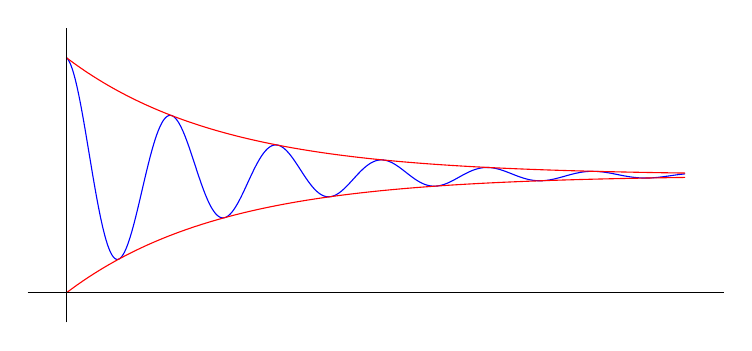
\begin{tikzpicture}
  \begin{axis}[xlabel=$t$,ylabel=$I$, xmin=-1, xmax=18, width=0.9\textwidth, height= 0.5\textwidth, axis lines = none,xtick=\empty, ytick=\empty]
    \addplot[samples = 500, domain=0:16, color=blue]{2*2.71^(-0.25*x)*cos(deg(2.3*x))};    %w=1.8, B=0.25, A=2
    \addplot[samples=500, domain=0:16, color=red]{2*2.71^(-0.25*x)};
    \addplot[samples=500, domain=0:16, color=red, label=test]{-(2*2.71^(-0.25*x))};
    \addplot +[mark=none, color=black] coordinates {(-1,-2) (17, -2)};
    \addplot +[mark=none, color=black] coordinates {(0,-2.5) (0,2.5)};
  \end{axis}
\end{tikzpicture}
\end{center}
\subsection*{Wechselstromkreise}
Es gilt, im Wechselstromkreis, Folgende eigenschaften
\begin{center}
\begin{tabular}{|p{4cm}|p{4cm}|}
  \hline
  \[\tikzfig{Widerstand}\]& \[V_R=-IR\]\\\hline
  \[\tikzfig{Kondensator}\]& \[V_C= \frac{Q}{C}\]\\\hline
  \[\tikzfig{Selbstinduktanz}\]& \[V_L = -L \frac{dI}{dt}\]\\\hline
\end{tabular}
\end{center}
\subsubsection{R-L Wechselstromkreis}
\begin{multicols}{2}
Sei ein Schaltkreis wir Rechts abgebildet ist.
\[\varepsilon(t)-L \frac{dI}{dt}-RI=0\]
\[L \frac{dI}{dt}+RI -\varepsilon_0 \cos\left( \omega t\right)\]
\vfill\null\columnbreak
\scalebox{1.3}{\tikzfig{R-LWechselSchaltkreis}}
\end{multicols}
Der ansatz $I(t)=I_0 \cos\left( \omega t+\alpha\right)$ kommt da wir eine  $I_0$ definieren durch:
\[I_0= \frac{\varepsilon_0}{\sqrt{R^2+\omega^2+L^2}}\]
Und wir können expandieren mit: ($\varepsilon_0$ ist spannung)
\[I_0= \frac{\varepsilon_0}{R}\cdot \cos\left(\alpha\right)\rightarrow \alpha\]
\subsubsection{R-C Wechselstromkreis}
\begin{multicols}{2}
Unser ansatz ist hier das gleiche und wir finden dass :
\[\tan(\alpha)= \frac{1}{\omega RC}\mspc I_0= \frac{\varepsilon_0}{R}\cos(\alpha)=\frac{\varepsilon_0}{\sqrt{R^2+\frac{1}{\omega^2C^2}}}\]
\vfill\null\columnbreak
\scalebox{1.3}{\tikzfig{R-CWechselSchaltkreis}}
\end{multicols}
\subsubsection{R-L-C WechselStromkreis}
%TODO Schema
Der Ansatz ist das Gleiche

\[\varepsilon(t)+\frac{Q}{C }-RI=0 \Longrightarrow -\frac{Q}{C }+R I-\varepsilon_0 \cos\left(\omega t\right)=0\]
Bei diesem Fall ist $\alpha$ von $\omega$ abhängig:
\[\tan(\alpha)=-\frac{\omega L }{R}=-\frac{1}{R }\left(\omega L-\frac{1}{\omega C}\right)\]
Und der Strom der durch den Kreis fliesst ist dann periodisch durch:
\[I=I_0 \cos\left(\omega t+\alpha\right)\]
Wobei unser $I_0$ eine Mischung von den R-L und R-C schaltkreisen ist, (die aber einen Anderen wert $L'$ oder $C'$ haben.)
\[I_0=\frac{\epsilon_0}{\sqrt{R^2+\left(\omega L-\frac{1}{\omega C }\right)^2}}\]
Wenn wir $I(\frac{\omega}{\omega_0})$ plotten, dann bekommen wir eine Resonanz kurve, wie bei der Mechanischen Schwingung, also wenn wir mit dei Resonanzfrequenz des Schaltkreises die Wechselstromquelle stellen, dann ist der Strom maximal. Die leistung ist auch so eine Kurve
\begin{figure}[h!]
\centering
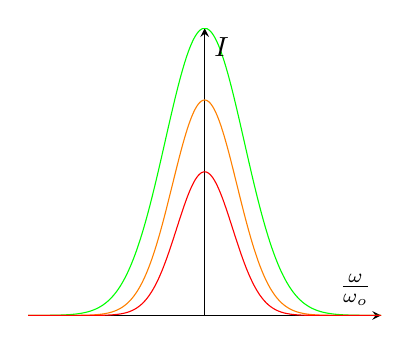
\begin{tikzpicture}
  \begin{axis}[xlabel=$\frac{\omega}{\omega_o}$, ylabel=$I$,axis lines = middle, xtick=\empty, ytick=\empty, width = 0.5\textwidth]
    \addplot[domain=-10:10, samples=500, color = green]{2*2.71^(-x^2*0.1)};
    \addplot[domain=-10:10, samples=500, color = orange]{1.5*2.71^(-x^2*0.15)};
    \addplot[domain=-10:10, samples=500, color =red]{2.71^(-x^2*0.2)};
  \end{axis}
\end{tikzpicture}
\end{figure}
\subsection*{Qualitätsfaktor}
Der Qualitätsfaktor $Q$ ist 
%TODO QUalitätsfaktor
\end{document}
